\documentclass{book}
\usepackage{epsf, a4, makeidx, Manu, hyperref}
\usepackage{palatino}
\usepackage{multicol}
\usepackage{graphicx} 
\usepackage[utf8]{inputenc}
\usepackage[french]{babel}

\usepackage{listings}
\lstloadlanguages{C}

\lstdefinelanguage{nasm}%
  {keywords={add, call, mov, iret, lcall, ljmp, jmp, push, pop, ret, shl, shr, xor},%
   otherkeywords={eax, ebx, ecx},%
   ndkeywords={ax, bx, cx},%
   sensitive=f,%
   morecomment=[l]{;},%
  }[keywords,comments,strings]%



% Insertion d'un lien vers les sources
%
% \fichier{chemin}{nom}{ext} (eg \fichier{lib}{console}{c})
%
\newcommand{\fichier}[3]{
\href{html/#2_8#3_source.html}{\lstinline!#1/#2.#3!}
(\href{html/#2_8#3.html}{\sc dox})
}

%-------------------------------------------------------------------------------
\title{Réalisation des prémices d'un noyau}
\author{Chaput Emmanuel}

\date{Version 0.00000001}

\makeindex

\begin{document}

\lstset{language=C,%
        basicstyle=\ttfamily,%
        keywordstyle=\bfseries,%
        ndkeywordstyle=\bfseries \underbar ,%
        identifierstyle=\em,%
        extendedchars}

\maketitle
\tableofcontents

%===============================================================================
%      Introduction
%===============================================================================
\chapter{Présentation générale}
%===============================================================================
%
%===============================================================================
\section{Introduction}

\subsection{Préambule}
   Ce document n'est constitué pour le moment que de quelques notes
que j'ai pu prendre en essayant de réaliser le début d'un truc qui pourrait
vaguement laisser penser que j'essaye de réaliser un noyau de système
d'exploitation. 

   Ces notes me sont purement personelles et je vous invite donc, qui que
vous soyez, arrêtez de lire ça ! Vous êtes encore là ? C'est pas sympa \ldots

%-------------------------------------------------------------------------------
%
%-------------------------------------------------------------------------------
\subsection{Présentation}

   Ce document rassemble quelques notes prises durant ma tentative de
dévelop\-pement de \manux (``Misérable Approximation de Noyau
Un*X''). Mon but en développant cette chose est uniquement de mieux
comprendre les problèmes liés à l'implantation d'un système
d'exploitation. Je n'ai en aucun cas comme objectif d'arriver à un
{\sc os} utilisable à d'autres fins que tester des mécanismes
systèmes. 

   De plus, je ne recherche absolument pas la performance dans le code 
que j'écris, mais plutôt la lisibilité et la compréhensibilité. Ça
peut ne pas sauter aux yeux dans les parties de code encore en
développement (c'est à dire partout pour le moment) \ldots 

%===============================================================================
%       Organisation générale
%===============================================================================
\section{Organisation générale}

   Comme tout système digne de ce nom, ManuX-32 définit un mode
utilisateur et un mode noyau. Il n'utilise pour l'instant pas les
différents modes fournis par le processeur, mais j'ai bon espoir pour
que cela arrive bientôt.

%-------------------------------------------------------------------------------
%   Structure du code
%-------------------------------------------------------------------------------
\subsection{Structure du code}

   Le code de ManuX est réparti dans quelques fichiers, eux-mêmes
organisés dans quelques répertoires.

   Au plus haut niveau, nous allons distinguer deux grandes parties
   que sont le ``code noyau'' et le ``code utilisateur''.
   
%...............................................................................
%
%...............................................................................
\subsubsection{Le code ``utilisateur''}

   Le code du monde utilisateur est confiné dans le répertoire {\tt
usr}.
  Les principaux fichiers de {\tt usr} sont les suivants

\begin{description}
   \item[{\tt unistd.c}] implante les principales fonctions (décrites
     dans {\tt include/unistd.h}) permettant l'accès aux fonctions du
     noyau. Comme nous le verrons, ce sont donc surtout des appels
     systèmes. 
   \item[{\tt stdio.c}] implante les principales fonctions (décrites
     dans {\tt include/stdio.h}) permettant de réaliser des
     entrées/sorties.
   \item[{\tt init.c}] implante le code de la première tâche lancée
     automatiquement par le noyau lorsqu'il est initialisé.
\end{description}

   La compilation du code utilisateur nécessite naturellement des
fichiers inclus. Ils se trouvent dans le répertoire {\tt
  usr/include}. Certains
     des fichiers, situés dans le répertoire {\tt include/manux} sont
     en fait des copies depuis l'arborescence du noyau. Ils sont mis à
     jour au travers de la cible {\tt usrinc} du {\tt Makefile
       principal}. Il s'agit de 

\begin{description}
   \item[{\tt config.h}] qui décrit la configuration du noyau, il est
     donc important de pouvoir en disposer dans le mode utilisateur
     afin de savoir ce qui est disponible ;
   \item[{\tt types.h}] qui définit les types utilisés dans le noyau ;
   \item[{\tt appelsystemenum.h}] qui donne les numéros des appels
     systèmes ;
   \item[{\tt string.h}] est là pour offir au mode utilisateur des
     fonctions présentes dans le noyau ({\tt memcpy()}, \ldots). Il
     n'est pas nécessaire que ce soit le même, mais cela évite de
     tenir à jour deux fichiers !
\end{description}

%...............................................................................
%
%...............................................................................
\subsubsection{Le code du noyau proprement dit}


\begin{description}
   \item[{\tt lib}]
   \item[{\tt noyau}]
   \item[{\tt i386}]
   \item[{\tt outils}]
   \item[{\tt boot}]
   \item[{\tt sf}]
   \item[{\tt doc}]
\end{description}

%-------------------------------------------------------------------------------
%   
%-------------------------------------------------------------------------------
\subsection{Configuration}

   La configuration se fait essentiellement au travers du fichier {\tt manux/config.h}.

   Certaines valeurs sont utilisées ailleurs que dans du C (dans du NASM,
ou directement dans le {\tt Makefile}) et une cible  {\tt make} est là
pour générer un fichier {\tt make.conf} qui contient ces
variables. Pour qu'elle fonctionne, il est impératif que ces macros
débutent par \lstinline!MANUX\_!

   D'autres valeurs doivent être déterminées durant la phase de
compilation (par exemple la taille du noyau). Elles sont donc
calculées par le programme {\tt outils/taillenoyau} et placées dans le
fichier {\tt taille.conf}.

%...............................................................................
%
%...............................................................................
\subsubsection{Le fichier {\tt include/config.h}}

   Il permet de choisir l'inclusion, ou non, de certines parties du
noyau, et parfois de les paramétrer.

%
%
%
\paragraph{Configuration du fichier de boot}

\begin{description}
   \item[{\tt MANUX\_TAILLE\_PAGE}]
   \item[{\tt MANUX\_NOMBRE\_PAGES\_SYSTEME}]
   \item[{\tt MANUX\_ADRESSE\_DEBUT\_TAS}]
   \item[{\tt MANUX\_NB\_MAX\_FICHIERS}]
   \item[{\tt MANUX\_CONSOLES\_VIRTUELLES}]
   \item[{\tt MANUX\_JOURNAL}]
\end{description}

%
%
%
\paragraph{Configuration de l'adressage du noyau}
\begin{description}
   \item[{\tt MANUX\_TAILLE\_PAGE}]
   \item[{\tt MANUX\_NOMBRE\_PAGES\_SYSTEME}]
   \item[{\tt MANUX\_ADRESSE\_DEBUT\_TAS}]
\end{description}

%
%
%
\paragraph{Configuration de l'affichage}

\begin{description}
   \item[{\tt MANUX\_CONSOLES\_VIRTUELLES}]
   \item[{\tt MANUX\_JOURNAL}]
\end{description}

%
%
%
\paragraph{Configuration du système de fichiers}

\begin{description}
   \item[{\tt NB\_MAX\_FICHIERS}]
\end{description}

%...............................................................................
%
%...............................................................................
\subsubsection{Le fichier {\tt make.conf}}

%...............................................................................
%
%...............................................................................
\subsubsection{Le fichier {\tt taille.conf}}


%-------------------------------------------------------------------------------
%   
%-------------------------------------------------------------------------------
\subsection{Organisation de ce document}

   Mon but est de décrire les choses de façon progressive, dans
l'ordre dans lequel je les ai faites, et dans l'ordre dans lequel il
me semble pertinent de les faire de sorte à construire progressivement
un noyau qui fonctionne.

   La section ``{\em Les outils de développement}'' décrit sommairement
les outils nécessaires à la compilation, le débogage et le lancement
de ManuX.

   La section ``{\em Le boot}'' montre comment faire en sorte que notre
code soit chargé en mémoire par le {\sc bios} de la machine puis
exécuté. C'est une partie assez technique, très spécifique au matériel
ciblé, et peu intéressante. Je vous autorise à la passer. À la fin de
cette partie, le code du noyau lui même commence à être exécuté, c'est
donc là que les choses deviennent croustillantes ! Mais c'est
également là que les ennuis commencent, \ldots

   Afin de pouvoir voir ce que nous faisons, une première activité va
consister à écrire du code pouvant afficher des choses à l'écran, nous
pourrons enfin avoir notre ``{\tt Hello world !}'' du noyau. Pour
cela, nous allons créer une ``console'' et une fonction
\lstinline!printk! dans la section ``{\em L'affichage}''.

   La section ``{\em Les appels systèmes}'' sera ensuite consacrée à
mettre en place le mécanisme permettant aux applications de
communiquer avec le noyau. Pour le moment, ce mécanisme n'est pas
nécessaire, un simple appel de fonction permet cela, mais lorsque nous
mettrons en place des mécanimes de protection, nous seronsbien
contents d'avoir fait les choses proprement !

   Dans la section ``{\em Un premier {\tt init}}'', nous alons écrire
un premier ``code utilisateur''

   Nous allons ensuite nous attaquer à un morceau assez conséquent :
la gestion de la mémoire qui sera décrite dans la section ``{\em La
  gestion de la mémoire}''. Nous ferons dans ManuX les choses aussi
simplement que possible. 
   


%===============================================================================
%
%===============================================================================
\chapter{Les outils}
%===============================================================================
%
%===============================================================================
\section{Les principaux outils}

   Le but de cette section est de décrire brièvement les outils
utilisés pour compiler et exécuter \manux.

   L'essentiel du code de \manux est écrit en C, et un peu
d'assembleur est nécessaire ici ou là, \ldots Le processus de
compilation est évidemment automatisé avec l'outil {\em make}. Je vais
décire sommairement cette étape dans la sous-section
\ref{subsection:compilation}.

   \manux peut ensuite être exécuté sur une machine réelle, mais il
est évidemment possible d'utiliser un émulateur. Nous évoquerons les
possibilités dans la sous-section \ref{subsection:execution}.

   Le débugage est un élément important dans la phase de développement
d'un logiciel, et il se révèle parfois un peu délicat lorsqu'il s'agit
de développer un noyau. Nous évoquerons des outils dans les
sous-sections \ref{subsection:debugage_interne} et
\ref{subsection:debugage_externe}.

%...............................................................................
%
%...............................................................................
\subsubsection{Le compilateur C}

   Le compilateur GCC est utilisé, la version 11.3.0 avec une cible
\lstinline!x86_64-linux-gnu! fonctionne parfaitement. Je n'ai jamais
eu de problème avec aucune version de GCC jusqu'à présent.

%...............................................................................
%
%...............................................................................
\subsubsection{L'assembleur}

   J'utilise \nasm \autocite{nasm-website}  pour les quelques fichiers
écrits en assembleur, dans sa version 2.14.
 
%-------------------------------------------------------------------------------
%
%-------------------------------------------------------------------------------
\subsection{La compilation}

   La commpilation générale du noyau est fondée sur l'outil {\tt
make}, et j'utilise la version 4.2.1 de \gnu {\tt make}.

%-------------------------------------------------------------------------------
%
%-------------------------------------------------------------------------------
\subsection{Les scripts}

   Quelques outils de scripts tels que {\tt awk} sont utilisés, rien
de très original, et tout système Linux correctement installé devrait
fournir ce qui est nécessaire.

%-------------------------------------------------------------------------------
%
%-------------------------------------------------------------------------------
\subsection{La gestion des fichiers {\sc iso}}

   Les fichiers {\sc iso} son générés par la commande {\tt
     grub-mkrescue} qui utilise {\tt xorriso}.
   
%-------------------------------------------------------------------------------
%
%-------------------------------------------------------------------------------
\subsection{L'exécution dans un émulateur}

   Bien sûr, l'idée n'est pas de faire fonctionner ManuX sur du
matériel réel, même si c'est tout à fait possible, mais plutôt dans un
émulateur.

   J'utilise pour cela \qemu dans sa version 3.1.0. On peut
également utiliser {\tt bochs} ainsi que VirtualBox.
   
%-------------------------------------------------------------------------------
%
%-------------------------------------------------------------------------------
\subsection{La documentation}

   La maigre documentation (que vous êtes  en train de lide) est
écrite essentiellement en LaTeX. N'importe quelle version convient
parfaitement.

   J'utilise également DoxyGen et mkdocs pour générer ensuite une
version navigable en ligne.

%===============================================================================
%
%===============================================================================
\section{Compilation de ManuX}

   Le {\tt Makefile} principal défini un certain nombre de cibles
utilisables pour compiler et exécuter ManuX.
   
%-------------------------------------------------------------------------------
%
%-------------------------------------------------------------------------------
\subsection{La création du noyau}

   Sans grande surprise, on compile avec la commande

\begin{lstlisting}
  make
\end{lstlisting}

  Différentes cibles peuvent être créées

\begin{itemize}
   \item {\tt manux} permet de compiler une image du noyau ;
   \item {\tt run} permet de lancer un émulateur (par défaut pour le moment c'est \qemu) ;
   \item {\tt clean} permet d'effacer tous les fichiers issus de compilation ;
   \item {\tt iso} permet de créer une image \iso.
\end{itemize}

%-------------------------------------------------------------------------------
%
%-------------------------------------------------------------------------------
\subsection{Gestion de configurations multiples}

   L'essentiel de la configuration de ManuX se fait dans le fichier
\fichier{include/manux}{config}{h}. Il est cependant possible de
demander à \make d'utiliser un fichier différent.

   Le répertoire {\tt multiconf} contient différents fichiers de
configuration. Chacun de ces fichiers permet alors de générer une
version différente de ManuX.

   Ainsi, le fichier \fichier{multiconf}{printk}{h} définit la
configuration permettant de compiler un noyau ManuX montrant
l'utilsation de {\tt printk}. On le compile de la façon suivante

\begin{lstlisting}
  make CFG=printk
\end{lstlisting}

   Il peut alors être exécuté par exemple avec

\begin{lstlisting}
  make run
\end{lstlisting}

%-------------------------------------------------------------------------------
%
%-------------------------------------------------------------------------------
\subsection{Création d'un fichier \iso}

   Il est également possible de créer un fichier \iso contenant une ou
plusieurs configuration de ManuX.

   Pour créer un fichier \iso contenant la version actuellement
définie dans le fichier \fichier{include/manux}{config}{h} on
utilisera simplement

\begin{lstlisting}
  make iso
\end{lstlisting}

   L'exécution pourra alors se faire via la commande

\begin{lstlisting}
  make runiso
\end{lstlisting}

   Il est également possible de générer un fichier \iso contenant
toutes les versions de ManuX décrites par les fichiers du répertoire
\lstinline!multiconf! de la façon suivante

\begin{lstlisting}
  make multiso
\end{lstlisting}

On l'exécutera de la même façon :

\begin{lstlisting}
  make runiso
\end{lstlisting}
   
%-------------------------------------------------------------------------------
%
%-------------------------------------------------------------------------------
\subsection{L'édition de liens}

   Afin d'assembler tous les éléments en un seul fichier
\lstinline!noyau.elf! qui pourra ensuite être utilisé par {\em
  Multiboot}, nous allons utiliser l'éditeur de liens \lstinline!ld!.
Le comportement de \lstinline!ld! est conditionné par un fichier qui
s'appelle un {\em linker script}. Un tel script décrit en particulier
comment les différentes sections des fichiers d'entrée sont disposées
dans le fichier de sortie et comment la mémoire est organisée.

%https://wiki.osdev.org/Linker_Scripts

Le code suivant montre un exemple simple de script :

\begin{lstlisting}
ENTRY(start)
SECTIONS {
    . = 1M 
    .boot :
    {
        *(.multiboot)
    }
    adresseDebutManuX = .;
    .text : {
       *(.text)
    }        
    .rodata : {
       *(.rodata)
    }
    .data : {
       *(.data)
    }
    .bss : {
       *(.bss)
    }
}
\end{lstlisting}

   Dans ce script, nous avous défini le nom du point d'entrée (ici {\tt
  start}), et nous avons décrit un certain nombre de sections avec
leur ordre d'apparition dans le fichier de sortie et leur
contenu. Vous remarquerez également que l'on utilise la notation
``{\tt .}'' pour spécifier l'adresse courante et que cette adresse
peut être consultée mais également modifiée. Ainsi la ligne {\tt . =
  1M} stipule que l'on se place ) l'adresse 1M. D'un autre côté la
ligne {\tt adresseDebutManuX = .} stipule que l'on enregistre dans la
variable {\tt adresseDebutManuX} la valeur de l'adresse courante
(celle du début de la section {\tt . text} donc).


%===============================================================================
%
%===============================================================================
\section{Exécution de ManuX}
\label{section:execution}

   Le but n'est évidemment pas de faire tourner cette merveille sur du
vrai matériel, mais plutôt dans un émulateur.

%...............................................................................
%
%...............................................................................
\subsection{L'émulateur Qemu}

   C'est maintenant \qemu \cite{qemu-website}  que j'utilise, par exemple de la façon
suivante
   
\begin{lstlisting}
   qemu-system-i386 -drive format=raw,file=manux,index=0,if=floppy -m 64M
\end{lstlisting}

  C'est d'ailleurs la commande que lance

\begin{lstlisting}
   make runfloppy
\end{lstlisting}

   Une autre façon de démarrer \manux est la suivante

\begin{lstlisting}
   qemu-system-i386 -kernel noyau.elf -m 64M
\end{lstlisting}

  C'est ce que fait la commande

\begin{lstlisting}
   make run
\end{lstlisting}

   Mais on préférera probablement passer par une image ISO :

\begin{lstlisting}
   qemu-system-i386 -m 64M -cdrom manux.iso
\end{lstlisting}

  C'est ce que fait la commande

\begin{lstlisting}
   make runiso
\end{lstlisting}

   De nombreuses options sont disponibles, mais ce n'est pas le moment
d'en parler !

%...............................................................................
%
%...............................................................................
\subsection{L'émulateur Bochs}

   J'utilisais initialement cet outil, mais les fichiers de
configuration ne semblent plus convenir aux dernières versions de
Bochs {} \cite{bochs-website} il faudrait les mettre à jour !

%===============================================================================
%
%===============================================================================
\section{Le débugage de ManuX}

%-------------------------------------------------------------------------------
%
%-------------------------------------------------------------------------------
\subsection{Le débugage ``interne''}
\label{subsection:debugage_interne}

   Ce que j'appelle ici le débugage interne, c'est tous les outils que
l'on peut utiliser dans le code lui-même pour essayer de comprendre ce
qu'il s'y passe.

   Nous avons pour le moment quelques outils de base, copieusement bugués
eux-mêmes (!).

%...............................................................................
%
%...............................................................................
\subsubsection{La fonction {\tt printk\_debug}}

   Elle permet de produire des messages d'erreur qui seront envoyés de
façon sélective en fonction de la valeur de \lstinline!masqueDebugage!
qui doit être construite dans {\tt manux/debug.h}.

%...............................................................................
%
%...............................................................................
\subsubsection{La macro {\tt assert}}

   Elle est définie dans le fichier \fichier{include/manux}{debug}{h}
et elle permet de vérifier {\em lors de l'exécution} qu'une propostion
est vérifiée ou non. Si elle ne l'est pas, un message est affiché.

%...............................................................................
%
%...............................................................................
\subsubsection{Le handler {\tt handlerPanique}}

   La fonction {\tt handlerPanique} est définie dans le fichier
\fichier{include/manux}{debug}{h} et permet d'afficher un état du
système qui peut être utile à des fin de débugage.

%...............................................................................
%
%...............................................................................
\subsubsection{Le fichier {\tt noyau/symbols}}

   Il va surtout nous servir pour aider au débugage externe, mais il
est généré à la compilation du noyau.
 
%-------------------------------------------------------------------------------
%
%-------------------------------------------------------------------------------
\subsection{Le débugage ``externe''}
\label{subsection:debugage_externe}

   Une technique pour débuguer est d'utiliser {\tt qemu} couplé avec
{\tt gdb}. Pour cela, je lance par exemple {\tt qemu} de la façon suivante

\begin{lstlisting}
   qemu-system-i386 -drive format=raw,file=manux,index=0,if=floppy  -rtc
base=localtime -m 64M -gdb tcp::1234  -S 
\end{lstlisting}

   Je lance ensuite {\tt gdb} dans un autre terminal avec un
\lstinline!.gdbinit! qui contient~:

\begin{verbatim}
  target remote :1234
  dir noyau
  dir lib
  file noyau/noyau.elf
\end{verbatim}

   La commande \lstinline!dir! permet de dire à {\tt gdb} où trouver
les fichiers sources et la command \lstinline:file: lui permet de
consulter le binaire du noyau pour y trouver l'adresse des fonctions
et variables (ici en fait, c'est une autre compilation du noyau au
format {\sc elf} !).

%...............................................................................
%
%...............................................................................
\subsubsection{Exécution}

   Quelques commandes de base pour l'exécution de code dans {\tt gdb}

\begin{itemize}
     \item {\tt {\bf r} un} permet de lancer l'exécution d'un
       programme (inutilisable ici étant donné notre fonctionnement :
       on débogue à distance) ;
     \item {\tt {\bf c} ontinue} permet de poursuivre l'exécution jusqu'au
       prochain point d'arrêt/bug/fin/\ldots ;
     \item {\tt {\bf s} tep} avance d'une instruction dans le code ;
     \item {\tt {\bf n} ext}
     \item {\tt {\bf b} reakpoint fonction}
     \item {\tt {\bf b} reakpoint fichier:ligne}
\end{itemize}

%...............................................................................
%
%...............................................................................
\subsubsection{Affichage des registres}

   Il peut être intéressant de consulter le contenu des registres

\begin{itemize}
     \item {\tt info registers} donne le contenu des principaux registres.
\end{itemize}

%...............................................................................
%
%...............................................................................
\subsubsection{Affichage des variables}

   {\tt Gdb} permet également de consulter le contenu des variables :

\begin{itemize}
   \item {\tt p toto} affiche le contenu de la variable {\tt toto}.
\end{itemize}

%...............................................................................
%
%...............................................................................
\subsubsection{Désassemblage du code}

    Une fonctionnalité intéressante est de pouvoir observer le code
assembleur, ce qui peut permettre de comprendre certains comportements
étranges, tels que les conséquences de choix d'optimisation du
compilateur :

\begin{itemize}
   \item {\tt disassemble fonc} affiche le code assembleur de la
     fonction {\tt fonc}.
\end{itemize}



%===============================================================================
%      Le démarrage
%===============================================================================
\chapter{Le boot}
%===============================================================================
%      Introduction
%===============================================================================
\section{Introduction}

   Nous allons ici voir comment en arriver à un noyau présent dans la
mémoire de la machine, prêt à être exécuté. La procédure peut varier
d'un système à l'autre : le code peut être sur un support amovible,
dans une zone mémoire non volatile, sur une machine distante, \ldots


   Dans les cas les plus simples, l'auteur du noyau n'a (presque) pas
à s'en préoccuper, dans les cas les plus tordus, il ou elle va devoir
(presque) tout faire. Nous décrirons ici deux variantes :

\begin{itemize}
   \item Nous commencerons par nous fonder sur une situation ``à
     l'ancienne'' avec un PC doté d'un lecteur de
     disquettes. Nous utiliserons alors le \bios du \pc
     pour charger le noyau en mémoire, lui passer quelques
     informations et le faire démarrer.

     Dans cette situation, nous devrons donc (presque) tout faire
     puisqu'il va falloir aller charger le noyau depuis la disquette
     vers la mémoire. Heureusement le \bios nous fourni des fonctions
     pour cela.

   \item Nous observerons ensuite des outils un peu plus modernes
     permettant de démarrer de façon un peu plus simple et plus
     indépendante du matériel sous-jacent.

     Dans cette situation, nous utiliserons par exemple {\tt grub} qui fera
     le travail de charger le noyau depuis le support (disque dur,
     \ldots) vers la mémoire. Nous aurons juste quelques informations
     à lui fournir.
  
\end{itemize}

%===============================================================================
%
%===============================================================================
\section{Démarage à partir d'une disquette}

   Nous allons donc devoir mettre en \oe{}uvre le boot du noyau dans
cette configuration. Pour cela, nous allons construire un fichier qui
sera placé sur une disquette à partir de laquelle notre système pourra
démarrer. Notons que nous utiliserons ici un émulateur comme Qemu ou bochs
auquel nous donnerons le chemin vers ce fichier et à qui nous
demanderons de démarrer depuis cette disquette. Mais nous pouvons
également copier ce fichier sur une disquette pour démarrer une vraie
machine.

   La première étape d'un tel démarrage est assuré par le système
lui-même : il s'agit de récupérer notre code sur la disquette, le
mettre en mémoire puis lui donner la main. C'est le BIOS qui va faire
cela. Malheureusement, son action est assez limitée, et il ne va
charger que 512 octets en mémoire. De ce fait,
notre code doit, d'une part être d'une taille inférieure à 512 octets
et d'autre part charger en mémoire le noyau lui-même.

   Nous allons donc construire un fichier composé essentiellement de
trois parties :

\begin{itemize}
     \item un {\em secteur de boot} (ou {\em bootsector}) sera un code
       de moins de 512 octets qui va s'occuper de charger le noyau ;
     \item un code d'initiaisation qui va préparer le terrain pour le
       noyau avant de démarrer celui-ci ;
     \item le noyau lui-même.
\end{itemize}

   Observons la structure de ce fichier pour ManuX puis regardons comment en
construire chaque partie.

%-------------------------------------------------------------------------------
%
%-------------------------------------------------------------------------------
\subsection{Construction du fichier de démarrage}

   Afin de permettre un démarrage ``à l'ancienne'' par un boot sur
disquette du \textsc{ pc}, nous allons donc construire une image de disquette
dont la structure est décrite par la figure suivante.

   Le code d'initialiation est ici nommé {\tt initmanux}. Je fais figurer
à la fin du noyau un fichier appelé {\tt ramdisk} qui peut être
présent et comporté un premier système de fichiers élémentaire.

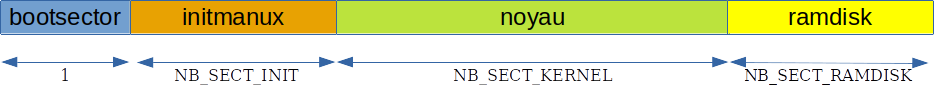
\includegraphics{images/image-disquette.png}

%\begin{figure}
%  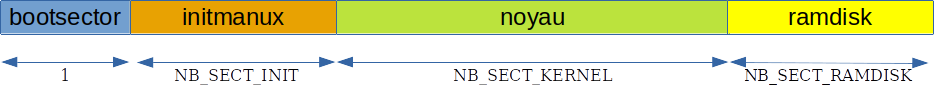
\includegraphics{images/image-disquette.png}
%\caption{\label{fig:image-disquette}Le fichier de démarage}
%\end{figure} 

   Ce que j'appelle ici le boot du système se passera donc en deux
temps. D'abord le secteur de boot est chargé en mémoire par le
\bios qui lui donne la main.

   Le secteur de boot  s'occupe alors de charger en mémoire le code
d'initialisation ainsi que le code du noyau. Il donne alors à son tour
la main à l'initialisation. Ce second élément réalise quelques
opérations puis démarre enfin le noyau.

   Si le secteur de boot et le code d'initialisation sont deux
éléments distincts, c'est pour deux raisons principales

\begin{itemize}
   \item d'une part le secteur de boot ne dispose que de 512 octets,
     si bien qu'il doit être réduit au  minimum ;
   \item chacun de ces deux éléments à un rôle bien spécifique
     (charger le code en mémoire et initialiser le système).
\end{itemize}

   Avant de regarder en détail comment ils sont mis en \oe{}uvre,
regardons les interactions entre les trois éléments.
   
%-------------------------------------------------------------------------------
%
%-------------------------------------------------------------------------------
\subsection{Liens entre les trois éléments}

   Les trois parties de codes évoquées ici (le secteur de boot, le
code d'initialisation et le noyau) ne sont pas liées entre elles (par
une édition de liens). Les appels de fonction, partages de variables,
\ldots {} sont alors à éviter car peu pratiques !

   Concrètement, il y a surtout deux ``appels de fonction'' à réaliser : 

\begin{itemize}
   \item le secteur de boot doit lancer le code d'initialisation ;
   \item le code d'initialisation doit démarrer le noyau.
\end{itemize}

   Pour cela, on va utiliser le fait que tous les éléments sont
placés à des adresses connues et faire un saut à ces adresses.
   
%-------------------------------------------------------------------------------
%
%-------------------------------------------------------------------------------
\subsection{Le secteur de boot}

   Lorsqu'on allume un \textsc{ pc} normalement configuré avec une disquette dans
le premier lecteur, le \textsc{ bios} charge le premier secteur de la diquette en
mémoire et l'exécute. En fait, il ne fait cela que si les deux derniers octets
de ce secteur contien\-nent la valeur magique {\tt 0xAA55}. Pour être
plus précis, c'est à l'adresse {\tt 0x7C00} que ce secteur est chargé.

   Un secteur étant composé traditionnellement de 512 octets, on ne
peut pas faire des folies avec le secteur de boot ! On va donc se
contenter de charger en mémoire d'autres secteurs du disque. Pour
cela, on peut utiliser le \bios et plus particulièrement
l'interruption 13h qu'il nous fournit pour manipuler les lecteurs.

   Le secteur de boot de ManuX est codé dans le fichier
\lstinline!boot/bootsector.nasm! et il est donc écrit en \nasm. Il est
très simple et se contente d'utiliser le \bios pour charger le
noyau en mémoire puis de faire un saut au début de la mémoire ainsi
initialisée.

   Il n'est pas très robuste, en particulier sur la taille attendue du
noyau et sur l'adresse à laquelle le placer !

   Concrètement, ce chargement se fait en deux phases :

\begin{itemize}
   \item Chargement du code d'initialisation : c'est le code qui va
     avoir pour rôle d'initialiser le système. Ce code est écrit en
     assembleur dans le fichier \lstinline!boot/init-manux.nasm!.
   \item Chargement du code du noyau : c'est tout le code de ManuX qui
     est ici chargé en mémoire. Il sera exécuté par le code
     d'initialisation. 
\end{itemize}

   Après ces deux chargements, le code du secteur de boot exécute le
code d'initialisation.

   Je ne décris pas plus ce code qui ne présente pas un intérêt
profond, les plus curieuses et curieux n'ont qu'à lire le code ! Vous
pourrez le trouver dans le fichier \fichier{boot}{bootsector}{nasm}.
   
%-------------------------------------------------------------------------------
%
%-------------------------------------------------------------------------------
\subsection{État de la mémoire après le chargement}

   L'état de la mémoire à la fin du boot est décrite par la figure
suivante. Les nombres sous les différentes zones expriment leur taille
en nobre de pages (la taille d'une page est de 4 Ko). Les macros sont
définies dans le fichier de configuration de \manux :
\fichier{include/manux}{config}{h}.

\includegraphics{images/etat-memoire-boot.png}

%\begin{figure}[htbp]
%\includegraphics[width=\textwidth]{etat-memoire-boot}
%\caption{\label{fig:etat-memoire-boot}État de la mémoire après le boot}
%\end{figure} 

   Une fois qu'il a terminé son travail, le code du secteur de boot
donne la main au code d'initialisation.
   
%-------------------------------------------------------------------------------
%      L'initialisation
%-------------------------------------------------------------------------------
\subsection{L'initialisation}

   Le "programme" d'initialisation est traditionnellement consacré à la détection
et à l'initialisation (original, vu son nom !) du matériel. Sur un \pc de
base, on peut là encore se faire aider du \bios. 

   En ce qui concerne \manux, cette phase d'initialisation va profiter
du fait qu'elle n'a pas les mêmes limites de taille que le secteur de
boot (un seul secteur comme le nom au singulier le suggère). On va
donc pouvoir y réaliser certaines actions un peu plus confortablement,
comme :

\begin{itemize}
   \item vérifier la mémoire disponible (cette information sera passée au
     noyau) ; 
   \item passer en mode protégé ;
   \item charger en mémoire un ramdisk qui nous permettra de jouer avec
    des systèmes de fichiers  sans avoir besoin d'implanter la gestion
    de matériel.
\end{itemize}

   Voyons rapidement quelques points.

%...............................................................................
%      Passage en mode protégé
%...............................................................................
\subsubsection{Passage en mode protégé}

   Les processeurs Intel démarre dans un mode de fonctionnement appelé
le {\em mode réel} (real mode). Dans ce mode, la mémoire est accédé de
façon linéaire. En mode protégé, l'utilisation de la mémoire est un
peu plus complexe (mais également plus puissante). Je ne vais pas
rentrer dans les détails ici, vous trouverez énormément de
documentation sur le sujet, par exemple les manuels Intel !

   Le basculement du mode réel vers le mode protégé n'est pas
immédiat, il nécessite un peu de travail.
   
%...............................................................................
%      Passage des informations au noyau
%...............................................................................
\subsubsection{Passage des informations au noyau}

   La plupart des informations recueillies par l'initialisation peuvent se
révéler particulièrement intéressantes pour le noyau. Il est donc important de
se définir un mécanisme permettant de faire passer ces informations depuis la
phase d'initialisation jusqu'au noyau.

   Nous allons utilise deux registres pour faire passer de
l'information au noyau :

\begin{itemize}
   \item Le registre \lstinline!eax! contiendra un ``nombre magique'',
     c'est-à-dire une valeur prédéfinie permettant au noyau
     d'identifier avec une bonne confiance le {\em bootloader}
     utilisé.
   \item Le registre \lstinline!ebx! contiendra l'adresse d'une
     structure dans laquelle seront enregistrées les différentes
     informations vraiment utiles pour le noyau.
\end{itemize}

   (Notons que ce choix (tout comme la structure qui va suivre) est
largement inspiré du fonctionnement de {\em Multiboot}). Nous aurons
donc par exemple la définition suivante dans le fichier
\fichier{include/manux}{multiboot}{h} 

\lstset{language=C}
\begin{lstlisting}
typedef struct _InfoSysteme {
   uint32_t flags;           // Pour compatibilité avec multiboot
   uint32_t memoireDeBase;   // En Ko
   uint32_t memoireEtendue;  // En Ko
   uint32_t peripheriqueDemarrage ;
   char *   ligneCommande;
} InfoSysteme;
\end{lstlisting}

   Naturellement, pour que tout cela fonctionne, il est nécessaire, à la fin
de la phase d'initialisation, d'initialiser correctement ces
registres. Voici donc par exemple à quoi peuvent ressembler les
dernières lignes de la phase d'initialisation :

\lstset{language=nasm}

\begin{lstlisting}
        ; On passe au noyau quelques infos
        ;---------------------------------
        mov eax, MANUX_INIT_MAGIC
        mov ebx, InfoSysteme

        ; Et c'est parti, on saute sur le noyau !
        ;----------------------------------------
        jmp MANUX_KERNEL_START_ADDRESS  
\end{lstlisting}

   Notons que, bien sûr, aucun contôle de type ne peut être fait entre les deux
phases et qu'il est donc important que le programmeur définisse de façon
cohérente la structure C et la zone mémoire gérée en assembleur.

%...............................................................................
%      Détection de la mémoire
%...............................................................................
\subsubsection{Détection de la mémoire}

   En ce qui concerne cette détection, nous allons encore une fois
utiliser un service du \bios, au travers de l'interruption 0x12 qui va
nous fournir ces informations.

   Vous trouverez le code correspondant dans le fichier
\fichier{boot}{init-manux}{nasm}. 


%===============================================================================
%
%===============================================================================
\section{Utilisation de {\em Multiboot}}

   Nous allons ici utiliser la spécification {\em Multiboot} définie
par la {\em Free Software Foundation} qui va nous permettre d'utiliser
les services d'outils tels que GRUB afin de grandement simplifier
le chargement du noyau de ManuX.

   Cela nous permettra également d'utiliser des outils un peu plus
modernes qu'un lecteur de disquettes et, par voie de conséquence, de
faire fonctionner ManuX sur autre chose que des machines virtuelles ou
hors d'age !

%-------------------------------------------------------------------------------
%
%-------------------------------------------------------------------------------
\subsection{Structure du fichier chargé par {\em Multiboot}}

   Nous devons construire un fichier qui sera fourni à {\em
Multiboot}.  Nous allons utiliser ici la version 1 de {\em Multiboot} et
non {\em Multiboot2}. On trouvera la spécification par exemple
\href{ici}{https://www.gnu.org/software/grub/manual/multiboot/multiboot.html}.

   Un tel fichier contient essentiellement notre noyau, mais doit avoir
une structure particulière afin d'être pris en charge~:

\begin{itemize}
   \item Il doit être composé d'un entête suivi d'un programme
     exécutable.
   \item L'entête, qui permet à l'outil de boot (comme {\sc grub})
     d'identifier le fichier, a une structure bien définie, que nous
     allons décrire ci dessous. Il doit être dans les 8192 premiers
     octets du fichier.
   \item Le programme exécutable peut être à n'importe quel format. Il
     doit évidemment être ``auto-suffisant'' (pas de librairies
     dynamiques !). Il doit pouvoir être positionné à n'importe quelle
     adresse physique en mémoire. 
\end{itemize}

   Le programme exécutable, c'est évidemment ManuX. Nous allons
décrire maintenant la structure de l'entête.
     
%-------------------------------------------------------------------------------
%
%-------------------------------------------------------------------------------
\subsection{Structure de l'entête}

   Le système {\em Multiboot} nécessite donc un entête devant le noyau
avec des caractéristiques bien définies.


%-------------------------------------------------------------------------------
%
%-------------------------------------------------------------------------------
\subsection{L'entête de ManuX}

   En ce qui concerne ManuX, il est
implanté dans le fichier \fichier{boot}{mb-manux}{nasm}.

   Ce fichier contient essentiellement quelques éléments permettant à
{\em Multiboot} de le reconnaitre puis du code permettant de démarrer
véritablement le noyau par un appel à la fonction \lstinline!_start()!
qui sera implantée dans le fichier \fichier{noyau}{main}{c}.

%-------------------------------------------------------------------------------
%
%-------------------------------------------------------------------------------
\subsection{Réalisation d'une image {\sc iso}}

   La cible {\tt iso}  du {\tt Makefile} principal permet de générer
un fichier {\sc iso} qui peut être utilisé pour démarrer ManuX sur une
machine physique ou virtuelle.

   La cible {\tt multiso} du {\tt Makefile} principal permet de
générer une image {\sc iso} intégrant un noyau pour chaque fichier de
configuration présent dans le répertoire {\tt multiconf}.

%===============================================================================
%
%===============================================================================
\section{Démarrage du noyau}

%-------------------------------------------------------------------------------
%
%-------------------------------------------------------------------------------
\subsection{Démarrage du noyau ({\tt noyau/main.c})}

   La dernière action du programme d'initalisation est donc l'exécution
de la fonction \lstinline!_start()!. Comme je l'ai dit précédemment,
il ne s'agit pas d'un appel de foncion C classique, puisque les deux
morceaux de code ne sont pas liés entre eux, mais d'un saut à
l'adresse de la fonction (le tout après avoir empilé les paramètres).

   Ceci termine donc la description de toute la quincailleire qui nous
permet d'arriver au début de l'exécution du code du noyau. Nous allons
commencer la description de ce dernier par la mise en place des outils
de base dont il aura besoin.

%-------------------------------------------------------------------------------
%
%-------------------------------------------------------------------------------
\subsection{Obtention des paramètres passés par le {\em bootloader}}



%===============================================================================
%      L'affichage
%===============================================================================
\chapter{L'affichage}
%===============================================================================
%      L'affichage
%===============================================================================
\section{Introduction}

   Une des premières choses à faire, afin de nous simplifier la vie
pour la suite du développement, est de se doter d'un service minimal
d'affichage. Nous allons donc mettre en place quelques outils très
simples fondés sur ce que nous founit le matériel.

   Nous ne nous intéresserons ici qu'à l'affichage des messages du
noyau, pas de ceux des éventuels processus utilisateurs. Nous
étendrons cependant un peu ces outils de sorte à nous permettre cela
par la suite.

   Nous allons procéder ici en trois étapes principales.

\begin{itemize}
   \item   Dans un premier temps, nous allons écrire le code
permettant un accès simple à l'écran et une gestion minimale de ce
dernier dans un module ``{\em Console}''. Cet outil est suffisant pour
que notre noyau soit capable de nous donner un signe de vie à
l'écran. Mais nous n'allons pas nous arrêter en si bon chemin !

   \item Nous pourrons alors écrire une fonction \lstinline!printk!
utilisable partout dans le noyau et chargée de mettre en forme des
messages riches et de les afficher sur la console,  \ldots{} ou ailleurs.

   \item   Nous construirons là-dessus un ``journal'' du noyau, c'est-à-dire
un outil permettant de rassembler et d'organiser les messages émis par
les différents sous-systèmes du noyau au travers de {\tt printk}.
Ils pourront être affichés sur la console, ou conservés pour être
stockés/traités d'une autre façon.
   Nous modifierons alors la fonction {\tt printk} de sorte à ce qu'elle
envoie au journal ce qui doit être affiché. C'est lui qui aiguillera
vers la bonne destination.

\end{itemize}

   L'avantage d'une telle structure est que nous pourrons la faire
évoluer. Nous pourrons par exemple créér des consoles virtuelles
fournissant le même service que notre outil de gestion de l'écran. Il
sera très simple de les intégrer dans le noyau. De même, nous pourrons
définir un affichage avec plusieurs niveaux d'importance des messages
qui pourront ensuite être aiguillés en fonction de leur criticité.

%-------------------------------------------------------------------------------
%
%-------------------------------------------------------------------------------
\section{Gestion de l'écran : la console}

   Les fichiers \fichier{include/manux}{console}{h} 
et \fichier{lib}{console}{c} définissent et implantent un outil de
gestion de base de la console.

   Nous allons pour le moment initialiser et utiliser une console
unique, que nous appellerons la ``console noyau''. Tous les messages
émis par le noyau y seront transmis.

   Nous allons définir essentiellement les éléments suivants

\begin{itemize}
   \item Le type \lstinline!Console! décrit ce qu'est une console.
   \item La fonction \lstinline!consoleInitialisation()! initialise le
     système de gestion de la console. Elle crée en particulier la
     console noyau. Cette fonction est invoquée une fois et une seule
     lors du démarrage du noyau.
   \item La fonction \lstinline!consoleAfficher()! permet d'afficher
     une chaîne de caractères sur la console.
\end{itemize}  

   Quelques autres fonctions, de moindre importance, sont également
définies.
   
%...............................................................................
%
%...............................................................................
\subsection{Fonctionnement de base}

   Il se trouve que l'écran d'un PC peut être utilisé en mode textuel
comme un simple tableau de caractères. Ce tableau est situé à une
adresse bien connue $a$ et contient $l$ lignes de $c$
caractères. Chaque caractère est codé sur deux octets : l'un définit
le code {\sc ascii} du caractère affiché et l'autre la couleur du
texte et du fond. 

%...............................................................................
%
%...............................................................................
\subsection{Définition du type {\tt Console}}

   Le type permettant de définir une console est défini dans le fichier
\fichier{include/manux}{console}{h}. Pour le moment nous ne créerons
qu'une console, mais lorsque nous allons introduire les consoles
virtuelles, nous étendrons ce type.

   Le type \href{html/console_8h_source.html#l00062}{\tt Console} est
donc très simple, il comprend quelques champs décrivant les
caractéristiques de l'écran (sa taille, l'adresse de la zone mémoire)
et l'état actuel de l'affichage (position du curseur et de
l'attribut).
   
%...............................................................................
%
%...............................................................................
\subsection{Initialisation de la console}

   L'initialisation du système de gestion de console (assurée par la
fonction \lstinline!consoleInitialisation()!) consiste essentiellement
en l'initialisation de la console noyau.

   La fonction d'initalisation de la console, implantée dans
\fichier{lib}{console}{c}, est elle aussi très simple. Elle se
contente d'une initialisation à des valeurs par défaut des champs du
type {\tt Console}.

   Nous n'utilisons ici pour le moment qu'une seule console, elle sera
définie comme une variable statique du fichier
\fichier{lib}{console}{c} et pourra être obtenue par la fonction {\tt
  consoleNoyau()} lorsque n'écessaire.

   En revanche, en prévision de la création de consoles virtuelles,
toutes les fonctions d'affichage prennent en première paramètre un
pointeur sur la console.

%...............................................................................
%
%...............................................................................
\subsection{Affichage sur la console}

   On construit ici en particulier la fonction suivante, chargée
d'afficher sur la console une chaîne de caractères passée en paramètre~:

\begin{lstlisting}
void afficherConsole(Console * cons, char * msg);
\end{lstlisting}

   Elle prend en paramètre une chaîne de caractères ``classique''
(terminée par un caractère nul) et l'affiche sur la console sans aucune
mise en forme.

   La gestion de la console est une des toutes premières choses
initialisées par le noyau, de sorte à pouvoir faire coucou dès que
possible.

%-------------------------------------------------------------------------------
%
%-------------------------------------------------------------------------------
\section{Un premier {\tt printk()}}

   Grâce à notre console, l'écriture de {\tt printk()} est assez
simple, puisque cette fonction n'a plus qu'à se préoccuper de créer
une chaîne de caractères et de la transmettre au journal (ou
directement à la console si on n'utilise pas le journal).

   Elle est définie dans le fichier \fichier{include/manux}{printk}{h}
   et mise en \oe{}uvre dans le fichier
   \fichier{noyau}{printk}{c}

   La fonction essentielle est bien sûr :

\begin{lstlisting}
   void printk(char * format, ...);
\end{lstlisting} 

   Dont le rôle est de mettre en forme une chaîne de caractères
qu'elle envoie ensuite à la console (ou au journal lorsque nous
l'aurons créé). Elle utilise pour cela le code suivant

\begin{lstlisting}
   afficherConsoleN(consoleNoyau(), chaine, indice);  
\end{lstlisting}

   Le paramètre \lstinline!indice! donne la longueur de la chaîne de
caractères \lstinline!chaine! qui est ainsi affichée sur la console du
noyau.
   
%-------------------------------------------------------------------------------
%
%-------------------------------------------------------------------------------
\section{Mise en place d'un journal}

   Le journal est spécifié dans le fichier
\fichier{include/manux}{journal}{h} et implanté dans le fichier
\fichier{lib}{journal}{c}.
   
   Nous allons définir un mécanisme de journal permettant de conserver
les messages transmis par le noyau. Pour le moment, notre journal se
contente de transmettre ces messages sur l'écran physique. Lorsque
nous aurons mis en place des outils de gestion mémoire, nous pourrons
étoffer ce mécanisme de journal.

   Le journal est implanté dans les fichiers
\lstinline!manux/journal.h! et \lstinline!lib/journal.c!. Il
propose essentiellement la fonction suivante

\begin{lstlisting}
   void journaliser(char * message); 
\end{lstlisting}

   Elle utilise la fonction \lstinline!afficherConsoleN()! pour
envoyer le message à la console.

   La fonction \lstinline!printk()! est alors modifiée pour utiliser la
fonction \lstinline!journaliser()! plutôt que passer directement par
la console.

   Évidemment, le journal est initialisé juste après la console.

%-------------------------------------------------------------------------------
%
%-------------------------------------------------------------------------------
\subsection{Introduction de plusieurs niveaux de messages}

   Maintenant que nous avons un système qui permet à tous les
sous-systèmes d'envoyer des messages, essentiellement {\em via} la
fonction \lstinline!printk()!, nous allons mettre en place un système
permettra de filtrer un peu tous ces messages.

   Pour cela, l'idée est d'utiliser la fonction \lstinline!printk()!
de la façon suivante

\begin{lstlisting}
   printk("{2} Un message\n");
\end{lstlisting}

   Ce sont les trois premiers caractères qui vont permettre de
réaliser cet aiguillage.

   C'est plus précisément le chiffre qui va permettre de définir le
niveau de criticité du message. Les valeurs suivantes sont définies
dans \fichier{include/manux}{journal}{h}~:

\begin{lstlisting}
#define MANUX_JOURNAL_NIVEAU_PANIQUE      0
#define MANUX_JOURNAL_NIVEAU_URGENCE      1
#define MANUX_JOURNAL_NIVEAU_CRITIQUE     2
#define MANUX_JOURNAL_NIVEAU_ERREUR       3
#define MANUX_JOURNAL_NIVEAU_ATTENTION    4
#define MANUX_JOURNAL_NIVEAU_NOTIFICATION 5
#define MANUX_JOURNAL_NIVEAU_INFORMATION  6
#define MANUX_JOURNAL_NIVEAU_DEBUGAGE     7
\end{lstlisting}  

   Les caractères qui encadrent le niveau de criticité permettent de
définir le comportement. Précisons ici en effet que, dès que nous
aurons mis en place des outils le permettant, nous allons associer un
fichier au journal. Ce fichier permettra par exemple de conserver les
messages du noyau, même après l'arrêt du système (ce qui est affiché
sur la console disparait, ce qui nest pas pratique pour une analyse a
posteriori).

La signification de ces caractères est alors la suivante~:
\begin{itemize}
   \item \lstinline![n]! et le message sera envoyé sur la console ;
   \item \lstinline!(n)! le message sera envoyé sur le fichier
     associé au journal ;
   \item \lstinline!{n}! le message sera transmis sur les deux
      destinations.     
\end{itemize}

   Le code de la fonction \lstinline!journaliser()! est donc modifier
en conséquence. Elle utiliser dans un premier temps la fonction
\lstinline!aiguillerMessage()! qui traite ce ``préfixe'' de sorte aue
le message soit transmis correctement, puis dans un second temps la
fonction \lstinline!journaliserNiveau()! qui transmet effectivement le
message à la (ou les) bonne(s) destination(s).

%-------------------------------------------------------------------------------
%
%-------------------------------------------------------------------------------
\section{Plus de souplesse avec les consoles virtuelles}

   Lorsque nous allons mettre en place la notion de tâches, il sera
intéressant d'attribuer à chacune d'entre elles une console virtuelle
potentiellement différente des autres. Nous pourrons ainsi basculer de
l'une à l'autre pour mieux distinguer ce qu'affiche chaque tâche.

%-------------------------------------------------------------------------------
%
%-------------------------------------------------------------------------------
\subsection{Utilisation des fichiers}



%===============================================================================
%      Gestion des interruptions
%===============================================================================
\chapter{Gestion des interruptions ({\tt interruptions.c interBasNiveau.nasm})}
%===============================================================================
%      
%===============================================================================
\section{Introduction}

   Les interruptions sont un outil fondamental dans la communication
d'un système avec son environnement. Leur gestion, nécessaire, soulève
quelques questions liées notemment au fil d'exécution.

%===============================================================================
%      
%===============================================================================
\section{Interruption, exception, code de traitement}

   Une interruption peut être vue commme la manifestation d'un
événement qui va perturber le fil d'exécution en cours sur un
processeur. Nous pouvons les classifier en deux catégories

\begin{itemize}
   \item {\bf Les interruptions asynchrones} (que nous appellerons
     simplement {\em interruptions}) sont le fait d'un élément
     extérieur au fil d'exécution en cours (une touche du clavier a
     été manipulée, une carte réseau a reçue une trame, \ldots). Nous
     parlerons également d'{\sc irq} (ou {\em Interrupt ReQuest} pour
     demande d'interruption).
   \item {\bf Les interruptions synchrones} (que nous appellerons {\em
     exceptions}) sont déclanchées par le processeur lui-même comme
     conséquence de l'exécution (ou de la tentative d'exécution) d'une
     instruction. 
\end{description}

   Une interruption, qu'elle soit synchrone ou non, aura pour
conséquence l'exécution par le processeur d'un code, appelé
{\em handler} d'interruption ou {\sc isr} (pour {\em Interrupt Service
  Routine}). Ce code est en charge de traiter l'interruption.

   Notons qu'il est également possible de générer volontairement une
interruption dans le code en cours d'exécution grâce à
l'instruction assembleur \lstinline!int n! (qui déclancher
l'interruption de vecteur \lstinline!n!). Nous utiliserons cette
option (ajouté au fait que le déclanchement d'une interruption à de
sconséquences plus complexes que le ``simple'' déroutement de
l'exécution) pour mettre en place le mécanisme des appels système.

%-------------------------------------------------------------------------------
%
%-------------------------------------------------------------------------------
\subsection{Vecteurs d'interruption, table d'interruption}

   Chaque interruption est associée à un {\em vecteur} qui va faire
office d'identifiant. C'est {\em via} ce vecteur que le
microprocesseur pourra déterminer où est le code du handler qu'il doit
exécuter lorsqu'une interruption est déclanchée.

   Concrètement, ce vecteur n'est pas directement l'adresse du
handler, mais l'indice dans une table, d'un descripteur du code du
handler. Il est ainsi possible d'avoir des descripteurs plus riches,
qui ne sont pas réduits simplement à l'adresse du code.

%...............................................................................
%
%...............................................................................
\subsubsection{La table d'interruptions x86}

   Sur l'architecture x86, cette table est appelée {\sc idt} (pour
{\em Interrupt Descriptor Table}) ; elle contient au maximum 256
descripteurs. Chacun de ces descripteurs est constitué de 8 octets qui
décrivent l'adresse du handler, le niveau de privilège requis, le type
d'interruption, etc \ldots

   Cette table peut se situer n'importe où en mémoire, c'est au
système d'exploitation de l'initialiser et d'informer le
microprocesseur de l'adresse à laquelle elle se trouve et de sa
taille. Le noyau utilise pour cela l'instruction {\tt lidt}.

%350 flux initial centrale vers 400 voire 450
%Actuellement 970 diplômés/an, c'est l'objectif pour 2030/31

%-------------------------------------------------------------------------------
%
%-------------------------------------------------------------------------------
\subsection{Les interruptions}

%-------------------------------------------------------------------------------
%
%-------------------------------------------------------------------------------
\subsection{Les exceptions}

   Les exceptions permettent donc de traiter un comportement erroné du
code en cours d'exécution (une tentative de division par zéro, un
accès à une zone mémoire protégée, \ldots).

   Elles sont traitées par le système de la même façon que les
interruptions déclanchées par du matériel. L'essentiel de ce qui est
dit ici pour les interruptions l'est donc en particulier pour les
exceptions.

%...............................................................................
%
%...............................................................................
\subsubsection{Les exceptions x86}

   Sur les processeurs Intel, les 32 premiers vecteurs sont attribués
aux exceptions.

%-------------------------------------------------------------------------------
%
%-------------------------------------------------------------------------------
\subsection{Les handlers d'interruption}

   Quelle que soit la nature de l'interruption, lorsqu'elle se
produit, un code spécifique (le ``handler'') est exécuté par le
processeur. Ce code doit donc effectuer certaines tâches

\begin{itemize}
   \item Sauvegarder l'état du microprocesseur de sorte à pouvoir
     ensuite reprendre l'activité qu'il menait.
   \item Intéragir éventuellement avec le matériel responsable de
     cette interruption pour le prévenir que le traitement est en
     cours. 
   \item Réaliser (ou reporter à un avenir proche) les opérations
     nécessaires suite à l'interruption : recevoir une trame sur une
     interface réseau par exemple.
   \item Restaurer l'état du microprocesseur qui reprendra où il en
     était avant l'interruption.
\end{itemize}
%-------------------------------------------------------------------------------
%
%-------------------------------------------------------------------------------
\subsection{Le traitement différé}

%-------------------------------------------------------------------------------
%
%-------------------------------------------------------------------------------
\subsection{Masquage}

   Une interruption peut éventuellement être  {\em masquée}, ce qui
signifie qu'elle ne sera pas délivrée au processeur, qui ne
s'appercevra donc pas qu'un événement s'est produit. Mais le masquage
d'une interruption n'empêche évidemment pas cet événement d'arriver !

%-------------------------------------------------------------------------------
%
%-------------------------------------------------------------------------------
\subsection{Traitement d'une interruption : partie haute et partie basse}

    Le traitement d'une interruption est donc en partie réalisé dans
un {\em handler}. Pour des raisons de simplicité, nous allons écrire
ces handlers en assembleur mais nous y utiliserons dès que possible
des fonctions C.

   Il est fondamental de comprendre que lorsqu'une interruption est
prise en compte par le processeur, le code qu'il était en train
d'exécuté est {\em interrompu} (surprise ?) pour exécuter le {\em
  handler}. Lorsque l'exécution de ce dernier s'achève, l'exécution du
code interrompu reprend son cours. Il est donc crucial que le {\em
  handler} ne réalise pas de modification du système qui rendrait
cette exécution incohérente (par exemple en supprimant une ressource
que ce code s'appétait à utiliser après s'être assuré de sa
disponibilité).

   Un autre élément fondamental est le fait que lorsqu'un handler
s'exécute, les interruptions ont inhibées et ne peuvent donc plus être
prises en compte\footnote{C'est un peu plus compliqué sur un système
  multiprocesseur.}. 

%===============================================================================
%      
%===============================================================================
\section{Le {\em Programmable Interrupt Controller}}

   Les interruptions peuvent arriver depuis plusieurs sources. Celles
provenant de périphériques (clavier, cartes réseau, \ldots) sont
éventuellement acheminées au travers de circuits spécialisés appelés
{\sc pic}.

   Le {\sc pic} est donc un circuit électronique permettant de gérer les
{\sc irq} provenant de l'environnement afin de les délivrer au
processeur (c'est en fait une fonction du {\em southbridge}).

   Je ne m'étalerai pas ici sur les différents types de {\sc pic} ni
sur leur fonctionnement. Ce qu'il est nécessaire de comprendre, c'est
qu'il existe donc un circuit avec lequel le processeur va devoir
dialoguer pour une partie de la gestion des interruptions.

   Nous verrons plus loin que ManuX gère le 8259A qui est un {\sc pic}
conçu par Intel.

%...............................................................................
%
%...............................................................................
\subsection{Le {\sc pic} Intel 8259A}

   Sur un (vieux) {\sc pc}, le {\sc pic} est un circuit Intel 8259A. Ce
circuit permet de gérer 8 types d'interruptions et on en utilise
plusieurs en cascade pour les additionner. Nous supposerons ici qu'il
y en a deux, le {\sc pic} 2 étant derrière le {\sc pic} 1 (en
``cascade'') pour un total de 15 interruptions.

   Ce circuit, donc on peut trouver la spécification
\cite{intel-8259a-spec} se programme au travers de deux registres

\begin{description}
    \item[Le registre de commande] accessible par le port 0x20 pour le
      circuit maître et 0xa0 pour le circuit esclave ;
    \item[Le registre de données] accessible par le port 0x21 pour le
      circuit maître et 0xa1 pour le circuit esclave.
\end{description}

   Une phase d'initialisation est nécessaire afin de configurer
correctement ces circuits.
   
   
%===============================================================================
%      
%===============================================================================
\section{Définition des handlers}

   Sur le 386, une table (l'{\sc idt} pour {\em Interrupt Descriptor Table})
définit le comportement à adopter pour chacune des 256 interruptions
et exceptionns. Cette table est enregistrée grâce à l'instruction
\lstinline!lidt!.

   Cette table contient des entrées de trois types différents

\begin{description}
   \item[Interrupt Gate]       
   \item[Trap Gate Descriptor]       
   \item[Task Gate Descriptor]       
\end{description}

%===============================================================================
%      
%===============================================================================
\section{Gestion dans ManuX}

   Observons ici comment tout cela est mis en place dans ManuX.

   Nous ne pouvons pas faire l'impasse sur un peu d'assembleur, si
bien que les fonctions ``bas niveau'' seront implantées dans les
fichiers {\tt manux/i386/interBasNiveau.h} et
\lstinline!i386/interBasNiveau.nasm!. Tout le reste sera en C dans {\tt
  manux/interruptions.h} et {\tt i386/interruptions.c}.

   Nous allons traiter séparément les trois types d'interruptions
suivants~:

\begin{itemize}
   \item les exceptions seront gérées ensemble via une fonction
     commune : \lstinline!gestionException()! ;
   \item les \irq seront traitées par une fonction commune, liée au \pic
     utilisé ;
   \item les exceptions logicielles seront elles aussi regroupées dans
     une seule fonction de traitement :
     \lstinline!gestionInterruption()!. 
\end{itemize}

   Dans les trois cas, la stratégie sera la même :

\begin{itemize}
   \item Nous allons définir en assembleur une fonction de traitement
     spécifique à chaque interruption. J'appellerai par la suite ces
     fonctions des {\em handlers d'interrruption}. Un handler
     d'interruption sera chargé d'invoquer une fonction d'aiguillage,
     écrite en C.
   \item Nous allons ensuite définir en C une fonction commune
     d'aguillage pour chaque type (\lstinline!gestionException()! pour
     les exceptions par exemple). Le rôle de cette fonction sera
     d'invoquer la fonction C chargée du traitement de l'interruption
     qui aura été déclenchée.
   \item Nous construirons enfin un tableau indexé par le numéro
     d'interruption et contenant un pointeur sur la fonction C de
     chaque interruption que l'on souhaite traiter spécifiquement.
\end{itemize}

   La figure suivante illustre cette logique.

\includegraphcs{images/interruptions.png}

   Observons maintenant ces différents éléments. Nous allons commencer
par écrire les handlers bas niveau en assembleur dans la prochaine
section.

   Nous observerons ensuite l'écriture en C  des fonctions de gestion
des interruptions.

%-------------------------------------------------------------------------------
%      
%-------------------------------------------------------------------------------
\subsection{Définition ``bas niveau'' d'un handler}

%...............................................................................
%
%...............................................................................
\subsubsection{Les exceptions}

   Nous allons observer à titre d'exemple les fonctions de gestion des
exceptions. Certaines exceptions empilent un code d'erreur de 32 bits
et d'autres ne le font pas. Comme nous faisons le choix de passer par
une fonction unique d'aiguillage, nous allons empiler une valeur nulle
sur 32 bits pour les exceptions qui n'utilisent pas de code d'erreur.

   Voici par exemple comment est écrit le gestionnaire bas niveau de
l'exception 0 (``division par zéro'') qui n'empile pas de code
d'erreur~:

\begin{lstlisting}{language=nasm}
golbal stubHandlerExceptionDivO
stubHandlerExceptionDivO :      ; Exception "division par zéro"
       push dword 0x0           ; On empile un "code"
       push dword 0x0           ; On empile le numéro de l'exception
       pushad                   ; sauvegarde des registres
       call gestionException    ; appel de la fonction d'aiguillage
       popad                    ; restauration des registres
       add esp, 0x08            ; on "dépile" le code et le numéro
       iret
\end{lstlisting}

   Et voici maintenant le code du gestionnaire bas niveau de
l'exception 0x0a (``TSS invalde'') qui empile l'indice du TSS en
erreur~:

\begin{lstlisting}{language=nasm}
global stubHandlerExceptionInvalidTSS
stubHandlerExceptionInvalidTSS :
       push dword 0x0a          ; On empile le numéro de l'exception
       pushad                   ; sauvegarde des registres
       call gestionException    ; appel de la fonction d'aiguillage
       popad                    ; restauration des registres
       add esp, 0x08            ; on "dépile" le code et le numéro
       iret
\end{lstlisting}

   Notons que lors d'une interruption, le microprocesseur empile les
valeurs de {\tt EFLAGS}, {\tt CS} et {\tt EIP} (voir par exemple
\cite{intel386pru1986} page 159).

   Si vous observez le fichier \lstinline!interBasNiveau.nasm!, vous
verrez que les 32 gestionnaires d'exception sont générées de la sorte
grâce à deux macros.

%...............................................................................
%
%...............................................................................
\subsubsection{Les \irq}

   En ce qui concerne les \irq, les choses sont encore plus simples
car toutes les interruptions ont le même comportement et les fonctions
sont générées (encore via une macro) avec des noms génériques.

   Voici par exemple à quoi ressemble le handler généré pour l'\irq
0~:
   
\begin{lstlisting}
stubHandlerIRQ0 :
   push dword 0            ; On empile le numéro de l'IRQ
   jmp  handlerIRQ

handlerIRQ :
   pusha                   ; On empile les registres
   call MANUX_HANDLER_IRQ  ; On appelle la fonction d'aiguillage
   popa                    ; On dépile les registres
   add esp, 4              ; Dépile le numéro d'IRQ
   iret
\end{lstlisting}

%...............................................................................
%
%...............................................................................
\subsubsection{Les interruptions logicielles}

   Une fois de plus, les handlers bas niveau sont générés par une
macro. Si nous observons le handler de l'interruption numéro 42, elle
ressemble au code suivant

\begin{lstlisting}
stubHandlerInt42 :
        push dword 42            ; On empile le numéro de l'interruption
	jmp  handlerInt
        
handlerInt :
	pushad                   ; Sauvegarde des registres
        call gestionInterruption ; Invocation de la focntion d'aiguillage
	popad                    ; Restauration des registres
        add esp, 4               ; On dépile le numéro d'interruption
        iret
\end{lstlisting}

   Regardons maintenant à quoi ressemblent les fonctions d'aiguillage.

%-------------------------------------------------------------------------------
%      
%-------------------------------------------------------------------------------
\subsection{Les fonctions d'aiguillage}

   Les fonctions d'aiguillage sont extrèmement simples : on utilise un
tableau dans lequel sont stoquées les pointeurs de fonction de chaque
interruption. La fonction d'aiguillage se contente donc d'invoquer la
fonction stoquée à l'indice correspondant.

   Pour les \irq, ce travail est réalisé par une fonction spécifique
au pilote du \pic.
   
%-------------------------------------------------------------------------------
%      
%-------------------------------------------------------------------------------
\subsection{Définition d'un handler en C}

   Nous pouvons par exemple écrire la fonction
\lstinline!handlerPanique! dont le rôle est d'afficher un message
permettant de déterminer la cause de l'interruption :

\begin{lstlisting}
void handlerPanique(uint32_t itNum, TousRegistres registres,
		    uint32_t eip, uint32_t cs, uint32_t eFlags)
{
   ...
}
\end{lstlisting}

   Nous la définissons avec les paramètres qui sont, dans l'ordre
inverse, les valeurs empilées par le processeur lors de l'interruption
puis par le handler ``bas niveau'' décrit ci-desssus.

   La structure \lstinline!TousRegistres!, décrite dans {\tt
manux/types.h}, permet de manipuler simplement l'ensemble des
registres.
   
%-------------------------------------------------------------------------------
%      
%-------------------------------------------------------------------------------
\subsection{Insertion d'un handler dans l'{\sc idt}}

   La procédure suivante initialise une entrée dans l'{\sc idt} :

\begin{lstlisting}{}
void positionnerHandlerInterruption(IDT idt, int i, Handler handler)
/*
 * Affectation du handler de l'interruption i
 */
{
   idt[i].itg.offsetFaible = ((uint32_t)handler & 0xFFFF);
   idt[i].itg.offsetFort = ((uint32_t)handler >> 16);
   idt[i].itg.parametres = 0x8E00;
   idt[i].itg.selSegment = SELECTEUR_SEGMENT_CODE;
}

\end{lstlisting}

   Elle sera donc appelée par la procédure d'initialisation de l'{\sc idt} pour
chacune des interruptions.

%-------------------------------------------------------------------------------
%      Initialisation de la table
%-------------------------------------------------------------------------------
\subsection{Initialisation de la table IDT}

   C'est la fonction C \lstinline!initialiserIDT()! qui est invoquée
par \lstinline!main()! pour initialiser la table.
   
   Nous avons maintenant tous les éléments pour construire notre {\sc
idt}. C'est le rôle de la fonction C \lstinline!initialiserIDT()!.
   
   Nous y positionnons donc tous les handlers sur le handler minimaliste
qui ne fait rien :

\begin{lstlisting}{}
   /* Comportement par defaut : on ne fait rien ! */
   for (i = 0; i < 256; i++) {
      positionnerHandlerInterruption(idt, i, stubHandlerNop);
   }
\end{lstlisting}

   Nous allons ensuite définir un handler un peu plus utile pour les
interruptions que peut nous générer le matériel

\begin{lstlisting}{}
   positionnerHandlerInterruption(idt, 0, stubHandlerPanique_0);
   positionnerHandlerInterruption(idt, 1, stubHandlerPanique_1);
   ...
\end{lstlisting}
   
   Nous pouvons enfin définir les handlers plus spécifiques

\begin{lstlisting}{}
   /* Le handler du timer */
   positionnerHandlerInterruption(idt, intTimer, stubHandlerTimer);

   /* Le handler du clavier */
   positionnerHandlerInterruption(idt, intClavier, stubHandlerClavier);
\end{lstlisting}

%...............................................................................
%
%...............................................................................
\subsection{Gestion du {\sc pic} Intel 8259a dans ManuX}

   Ce circuit est géré au travers de fonctions définies dans {\tt
include/manux/intel-8259a.h} et implantées dans {\tt
     i386/intel-8259a.c}.

   L'objectif est assez simple : fournir (aux drivers des matériels
utilisant un mécanisme d'interruption) une interface générique,
c'est-à-dire indépendante du {\sc pic} utilisé. Nous allons donc
définir quelques fonctions de base permettant à ces drivers de
s'interfacer avec le système d'interruption. Si on souhaite utiliser
un autre circuit {\sc pic} (par exemple un  {\sc apic}), il
``suffira'' de réécrire ces fonctions, il n'y aura pas besoin de
modifier le code des nombreux drivers (au moins deux, rendez-vous
compte du boulot !) qui l'utilisent.

   Le principe général consiste à définir un handler d'interruption
unique qui va prendre en charge toutes les interruptions générées au
travers du {\sc pic}. Ce handler traitera les aspects spécifiques au
{\sc pic} puis invoquera le handler de chacun des ``clients''
c'est-à-dire des drivers des matériels qui sont à la source des
interrruptions.

   Décrivons les fonctions principales. Vous retrouverez leur code
dans {\tt i386/intel-8259a.c}.

\paragraph{\tt i8259aInit} permet d'initialiser
les circuits (le {\sc pic}) et de les configurer pour que les
interruptions générées utilisent une plage de numéros commençant à une
valeur passée en paramètre.
\paragraph{\tt i8259aAjouterHandler} permet d'associer une fonction
et des données à une {\sc irq}. C'est par le biais de cette fonction
qu'un client va se faire connaître auprès de notre système.
\paragraph{\tt i8259aGestionIRQ}


\chapter{La communication avec le monde utilisateur}
%===============================================================================
%      Les appels système
%===============================================================================
\section{Les appels systèmes}

   Les appels systèmes constituent une part importante de l'interface
entre le noyau et les applications. Dans ManuX, le choix a été fait
d'implanter ce mécanisme au travers d'une interruption. C'est une
technique classique (utilisée par exemple par Linux).

   Leur mise en \oe{}uvre passe par plusieurs étapes que je vais
détailler ici. L'objectif d'un appel système est d'offrir à une
application utilisateur un service qui ne peut être rendu que part le
noyau. Pour des raisons de confort d'utilisation, ces services sont
rendus sous la forme de fonctions classiques, comme une librairie
traditionnelle. Pour en arriver là, nous pouvons distinguer quatre
étapes

\begin{itemize}
   \item L'application utilise une fonction C pour invoquer un appel
     système. Le code de cette fonction doit donc être construit de
     sorte à préparer puis mettre en \oe{}uvre la sollicitation du
     service auprès du noyau (par le biais d'une interruption ici).
   \item L'interruption est déclanchée et le code du handler de cette
     interruption est exécuté.
   \item Le handler va devoir déterminer quelle est la fonction du
     noyau qui doit être utilisée pour rendre le service voulu à
     l'application.
   \item La fonction en question va être exécutée et le service fourni
     à l'application.
\end{itemize}

   Nous allons maintenant décrire la mise en \oe{}uvre de ces étapes
en prenant comme exemple un appel système qui nous permettra d'envoyer
un message sur la console. Nous pourrons ainsi écrire un
\lstinline!printf! pour les applications !

%-------------------------------------------------------------------------------
%      Définition de l'interface
%-------------------------------------------------------------------------------
\subsection{Définition des éléments communs noyau/application}

   Le fichier \fichier{manux}{appelsystemenum}{h} donne en particulier les
numéros des différents appels systèmes. Il doit donc absolument être
commun au noyau et aux ``applications'' (voir la documentation sur
l'espace utilisateur).

%-------------------------------------------------------------------------------
%      Définition de l'interface
%-------------------------------------------------------------------------------
\subsection{Définition de l'interface}

   Ce que j'appelle interface est la signature de la fonction
directement utilisable dans une application pour invoquer un appel
système.

   Cette interface est donc décrite côté applications, dans les
fichiers de {\tt usr}.
   
   Des macros ont été créées dans le fichier \fichier{usr/include/manux}{appelsysteme}{h}
pour simplifier une telle définition. Ce
sont par exemple les ``fonctions'' \lstinline!appelSysteme0!,
\lstinline!appelSysteme1!, \ldots 

   On utilisera donc une telle macro chaque fois qu'il sera nécessaire
de définir un nouvel appel système. C'est ainsi que dans le fichier
\lstinline!usr/include/unistd.h! on trouve par exemple :

\begin{lstlisting}
appelSysteme2(NBAS_AFFICHER, int, afficherConsole, void *, int);
\end{lstlisting}

   Cette ligne défini donc la fonction \lstinline!afficherConsole()!
qui va permettre à une application d'envoyer un message sur la console.

%-------------------------------------------------------------------------------
%      Ecriture de l'appel système
%-------------------------------------------------------------------------------
\subsection{Écriture de l'appel système}

   La partie la plus importante est naturellement d'écrire le code de
l'appel système. Celui-ci consiste simplement en une fonction C
classique (qui en utilise éventuellement d'autres, naturellement). La
seule contrainte étant que si cette fonction a des paramètres, le
premier d'entre eux (qui ne présente aucun intéret pour le
programmeur) doit être de type \lstinline!ParametreAS!.

   Ce paramètre sert uniquement a ``recadrer'' les paramètres suivants 
dans la pile suite aux décalages induits dans celle-là par les appels
successifs à l'interface de l'appel système, à l'interruption, et à
l'appel système lui-même d'une part, et à la sauvegarde des registres
d'autre part.

   Observons par exemple le code permettant la mise en \oe{}uve de
l'appel système \lstinline!ecrireConsole!. Il se trouve dans le
fichier {\tt lib/console.c} :

\begin{lstlisting}
/**
 * L'implantation de l'AS ecrireConsole
 */
int sys_ecrireConsole(ParametreAS as, void * msg, int n)
{
   assert(tacheEnCours != NULL);
   Console * cons = tacheEnCours->console;
   
   assert(cons != NULL);
   afficherConsoleN(cons, msg, n);

   return n; 
}
\end{lstlisting}

   Bien sûr, cette fonction utilise le code de manipulation de la
console déjà écrit.   

%-------------------------------------------------------------------------------
%      Enregistrement de l'appel système
%-------------------------------------------------------------------------------
\subsection{Enregistrement de l'appel système}

   L'enregistrement de l'appel système dans le système d'exploitation est
réalisé par une invocation de la fonction suivante, définie dans {\tt
appelsysteme.h} et codée dans {\tt noyau/appelsysteme.c} :

\begin{lstlisting}{}
int definirAppelSysteme(int num, void * appel);
\end{lstlisting}

   où 

\begin{description}
   \item[\lstinline!num!] est le numéro de l'appel système enregistré ;
   \item[\lstinline!appel!] est la fonction de traitement de cet appel
système.
\end{description}

   Le travail de cette fonction est donc simplement de placer dans la
table des appels systèmes (\lstinline!vecteurAppelsSysteme!) la
fonction de traitement de cet appel système.

   C'est donc ici la ``partie noyau'' qui est réalisée, c'est-à-dire
la définition des actions à mener lorsque l'appel système est invoqué.

   Nous trouvons par exemple dans la fonction
\lstinline!initialiserAppelsSysteme()! du fichier {\tt
  noyau/appelsysteme.c} la ligne de déclaration de notre appel système
\lstinline!ecrireConsole! :

\begin{lstlisting}{}
void initialiserAppelsSysteme()
{
   ...
  
   /* Envoyer une chaine de caracteres sur la console */
   definirAppelSysteme(NBAS_ECRIRE_CONS, sys_ecrireConsole);

   ...
}
\end{lstlisting}{}



%===============================================================================
%
%===============================================================================
\section{Un premier {\tt init}}

   Nous avons désormais tout ce qu'il nous faut pour mettre en place
du ``code utilisateur'', c'est-à-dire un code qui ne fait pas partie
du noyau, mais qui consitue une application utilisant les services du
noyau au travers des appels système.

   Attention, comme mentionné précédemment, les ``applications''
s'exécutent pour le moment dans le même mode que le noyau.

%===============================================================================
%      La gestion des tâches
%===============================================================================
\chapter{Les tâches}
%===============================================================================
%      Gestion des tâches
%===============================================================================
\section{Gestion d'une tâche}

   Nous disposons désormais du minimum permettant d'exécuter quelques
instructions et d'en voir les conséquences à l'écran. Je vous propose
donc de mettre en place la notion de {\em tâche} qui nous permettra de
faire avancer ``en même temps'' plusieurs activités. ManuX devient
donc à partir de maintenant un système multitâche.

   Attention, pour le moment, ce ne sera que du multitâche
collaboratif. En effet, nous n'allons pas encore mettre en place du
multitâche {\em préemptif}, ce qui signifie que une tâche ne rendra la
main (enfin, le processeur) que lorsqu'elle en aura envie !

   De plus, nous ne nous intéressons pas non plus à l'ordonnancement,
et mettrons en place un simple {\em round robin}.

%-------------------------------------------------------------------------------
%      Définition d'une tâche
%-------------------------------------------------------------------------------
\subsection{Définition d'une tâche}

   La structure d'une tâche est définie dans le fichier {\tt
manux/tache.h} au travers d'une struture \lstinline!Tache!. Afin de
nous simplifier la vie, nous allons utiliser dans ManuX l'aide
proposée par les processeurs Intel\footnote{Les systèmes récents, pour
  des raisons de performances, n'utilisent pas ces fonctionnalités.}.

   De ce fait, la structure \lstinline!Tache! contient des champs liés
au processeur et des champs purement liés au noyau.

%...............................................................................
%
%...............................................................................
\subsubsection{Champs liés au noyau}

%...............................................................................
%
%...............................................................................
\subsubsection{Champs liés au processeur}

\begin{itemize}
   \item \lstinline!IntelTSS tss! qui permet, comme son nom laisse à
penser, de stoquer les informations relatives à l'état de la tâche au
niveau du processeur ({\sc tss} pour {\em Task State Segment}). On
trouvera des informations sur ce champs dans les documentations Intel.
Dans ManuX, une initialisation minimale est faite de cette structure
lors de la création d'une tâche dans \lstinline!creerTache!.

   \item \lstinline!uint16 indiceTSSDescriptor! représente l'indice,
dans la {\sc gdt}, du {\em {\sc tss} Descriptor} de la tâche. C'est
par un \lstinline!ljmp! vers ce champs que l'on va activer la tâche.

   \item \lstinline!DescriptorTable * ldt! est la table locale de
decripteurs associée à cette tâche.
\end{itemize}

%Ètant donnée la gestion limitée de la mémoire à ce niveau du
%système, les structures définissant une tâche sont placées dans une
%même page mémoire et organisées comme représenté sur la figure
%\ref{Figure:PageTache}.
%
%\begin{figure}[htbp]
%\epsfxsize=5cm
%$$
%\epsfbox{PageTache.eps}
%$$
%\caption{\label{Figure:PageTache}Structure d'une page de tâche}
%\end{figure} 
x
%...............................................................................
%
%...............................................................................
\subsubsection{Les descripteurs de tâche Intel}

   Le {\em Task State Segment} ({\sc tss}) des processeurs Intel
permet de stoquer et de manipuler les informations relatives à une
tâche. Dans ManuX, une structure est définie permettant de décrire
dans le noyau le {\sc tss} de chaque tâche : la structure
\lstinline!IntelTSS! est définie dans
\lstinline!manux/tache.h!

%-------------------------------------------------------------------------------
%      Création d'une tâche
%-------------------------------------------------------------------------------
\subsection{Création d'une tâche}

%-------------------------------------------------------------------------------
%      Basculement vers une tâche
%-------------------------------------------------------------------------------
\subsection{Basculement vers une tâche}

   En ce qui concerne le basculement d'une tâche à l'autre, nous
allons profiter des mécanismes fournis par les processeurs Intel au
travers de l'instruction {\tt ljmp}. L'{\em Indirect far JMP} permet
en effet de faire un basculement de tâche lorsque l'argument qui lui
est passé, sur 48 bits (oui madame, 6 octets !) est constitué d'un
sélecteur de segment (sur 16 bits) qui référence un {\sc tss} puis
d'un {\em offset} (qui ne sera pas utilisé pour le coup !).

   Bref, le basculement d'une tâche vers une autre se résume à une
instruction de saut !

%-------------------------------------------------------------------------------
%      Destruction d'une tâche
%-------------------------------------------------------------------------------
\subsection{Destruction d'une tâche}

%===============================================================================
%      Gestion des listes de tâches
%===============================================================================
\section{Gestion des listes de tâches}

   Il est évidemment important de ne pas perdre trace des tâches
créées sur le système ! Nous allons pour cela les placer dans des
listes.

   La structure \lstinline!ListeTache! permettant cela est définie
dans le fichier \fichier{manux}{listetaches}{h}. Il est extrèmement
simple (liste simplement chaînée), donc je ne le détaille pas ici.

   Une première liste est définie permettant de conserver toutes les
tâches du système. Chaque tâche créée (et non encore détruite) sera
donc présente dans cette liste.

   D'autres listes seront créées permettant de stoquer les tâches en
fonction de leurs activités. Une liste contiendra par exemple les
tâches prêtes à être exécutées. D'autres listes contiendront les
tâches en attente d'un événement spécifiques (typiquement la
disponibilité d'une ressource).
   
\includegraphcs{images/exemple-taches.png}

%-------------------------------------------------------------------------------
% Allocation des éléments de liste
%-------------------------------------------------------------------------------
\subsection{Allocation des éléments de liste}

   Bon, là il faut qu'on parle d'un truc dont je ne suis pas très fier
\ldots

   Pour ne pas avoir à s'em\lodts bêter ici avec de la gestion
dynamique de mémoire, et sûrement aussi dans un intérêt pédagogiqe
évident, j'ai fait le choix de positionner les cellules impliquées
dans la gestion des listes dans la page mémoire qui est allouée pour
chaque tâche.

        
 


%===============================================================================
%      La gestion de la mémoire
%===============================================================================
\chapter{La mémoire}
%===============================================================================
%      Gestion de la mémoire
%===============================================================================
\section{Gestion de la mémoire}

   La gestion de la mémoire est une fonction essentielle d'un système
d'exploitation. Nous allons dans un premier temps jeter un coup
d'\oe{}uil rapide à la gestion de la mémoire vue par Intel.

   Il y a plusieurs concepts à intégrer. Cela peut sembler complexe,
mais en prenant un peu de temps, vous vous rendrez compte qu'il n'y a
rien de méchant !

   Le premier est la {\em segmentation}. Pour faire simple,
imaginez-vous fin des années 70 avec un microprocesseur dont les
registres sont sur 32 bits. Comment adresser plus de 64 Ko ? La
segmentation consiste à utiliser deux registres pour composer une
adresse de plus de 32 bits. Nous allons voir que ce concept a été
enrichi et utilisé à d'autres fins.

   Le second est la {\em pagination}. L'idée ici est de découper la
mémoire en {\em pages} de taille fixe. Chaque page pourra être dotée
de propriétées qui lui sont propre. La pagination va nécessiter la
mise en place d'un certain nombre de tables d'indirection, ce qui peut
sembler un peu lourd, mais qui va en particulier permettre de la
mémoire virtuelle, de l'isolation entre les tâches, \ldots

%-------------------------------------------------------------------------------
%
%-------------------------------------------------------------------------------
\subsection{La segmentation}

   Essayons de comprendre ce qui se passe lorsqu'une instruction du
processeur doit manipuler une adresse. Nous nous en tiendrons ici à
l'architecture des Intel 386.
   
   Imaginons par exemple une instruction qui doit aller lire ou écrire
un octet en mémoire ou encore une instruction qui effectue un saut
vers une nouvelle zone de code. Une telle instruction va donc exprimer
explicitement une adresse, appelée {\em adresse logique}. Cette
adresse logique est composée de deux parties : un {\em segment}, et un
{\em offset}.

   Le segment est une partie de la mémoire, et l'offset un déplacement
dans le segment, comme l'illustre la figure \ref{Fig-1}. On
peut donc voir ça comme une découpe de la mémoire 
en zones (ou segments) logiques et/ou comme une façon d'accéder à des
adresses plus élevées que ce que permet la taille des registres.

%\begin{figure}[htbp]
%$$
%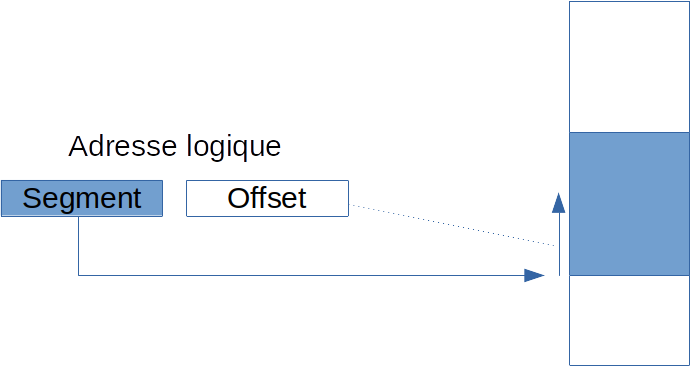
\includegraphics[width=0.4\textwidth]{adresse-logique}
%![](adresse-logique.png){}

\begin{figure}[htbp]
\begin{center}
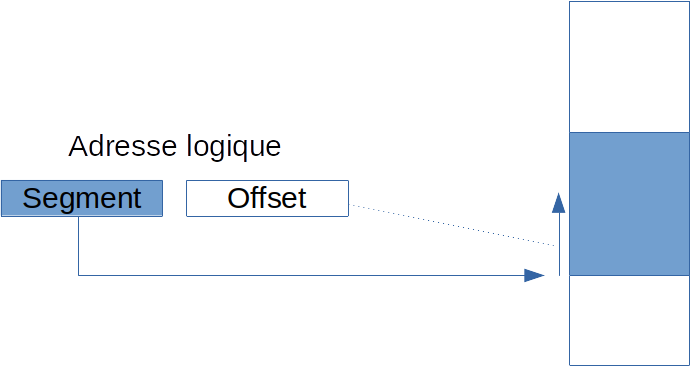
\includegraphics[width=0.6\textwidth]{adresse-logique.png}
\caption{\label{Fig-1}Adresse logique}
\end{center}
\end{figure} 

   Le segment est contenu dans un registre qui peut être fourni
explicitement ou implicitement par l'instruction. Il donne donc
l'adresse de la zone mémoire que l'on appelle un segment. Sauf que
c'est malheureusement un peu plus complexe que ça ! Un segment n'est
en effet pas décrit uniquement par son adresse (et quand bien même !
On a dit qu'un registre ne pouvait pas contenir une adresse entière).

   En fait, le registre en question permet d'accéder à un {\em
descripteur de segment}. C'est évidemment ce dernier (que nous
allons décrire par la suite) qui donne, entre autres, l'adresse du
segment. La figure \ref{Figure:addlogsel} illustre cette indirection.

\note{
\begin{figure}[htbp]
$$
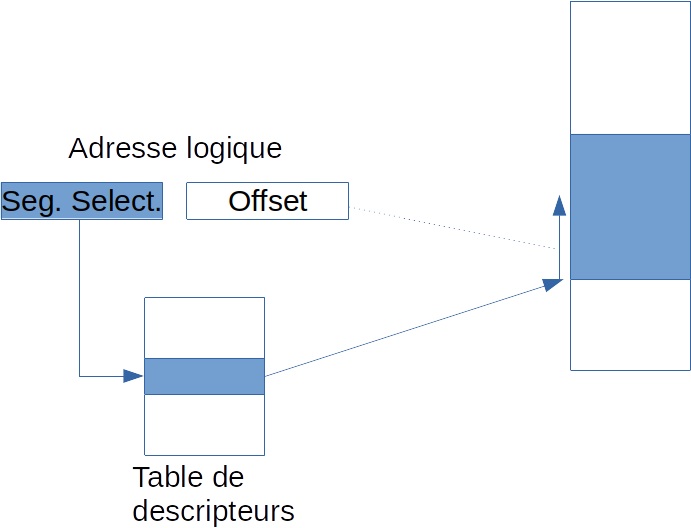
\includegraphics[width=0.4\textwidth]{adresse-logique-sel}
$$
\caption{\label{Figure:addlogsel}Adresse logique et sélecteur de segment}
\end{figure} 
}

%-------------------------------------------------------------------------------
%      Segmentation
%-------------------------------------------------------------------------------
%\subsection{La segmentation sur les processeurs Intel}

   Dans les versions antérieures de ses processeurs (et dans le mode
``réel'' du 386), la mémoire est découpée logiquement en {\em
segments}. Une adresse est alors désignée par un couple composé d'un
{\em registre de segment} et d'un {\em registre d'offset}.

   Concrètement, la taille d'un segment est de 64 Ko (puisque le
registre d'offset est sur 32 bits).

   À partir du 286 (si je ne me trompe pas), en mode dit ``protégé'', un
registre de segment devient une référence vers un {\em descripteur de
segment}. Ce dernier permet une gestion beaucoup plus évoluée de la
mémoire.

   Les descripteurs de segment sont rassemblés dans une table, la {\sc 
gdt} ({\em {\bf G}lobal {\bf D}escriptor {\bf T}able}) ou la {\sc ldt}
({\em {\bf L}ocal {\bf D}escriptor {\bf T}able}). Un registre de
segment représente alors simplement le décalage d'un descripteur dans
la table.

   Lorsque l'on utilise un registre de segment, il contient donc
en fait l'adresse (dans la {\sc ldt} ou dans la {\sc gdt}) d'un
descripteur de registre. Ce descripteur contient lui-même l'adresse du
segment.

%...............................................................................
%      Les descripteurs de segment
%...............................................................................
\subsubsection{Les descripteurs de segment}

   La figure \ref{Figure:DescrSegment} montre la structure d'un
descripteur de segment.

\note{
  \begin{figure}[htbp]
$$
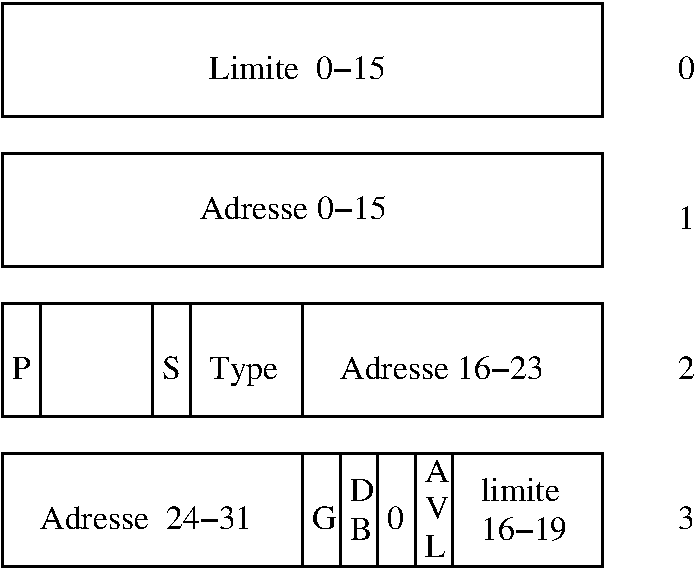
\includegraphics[width=0.3\textwidth]{DescrSegment}
$$
\caption{\label{Figure:DescrSegment}Structure d'un descripteur de segment}
\end{figure} 
}
   Dans ManuX, la fonction suivante crée un descripteur de segment et
l'ajoute dans la {\sc gdt} ou la {\sc ldt} passée en paramètre :

\begin{lstlisting}{}
int setDescripteurSegment(DescriptorTable * dt,
                          uint32 adresse, uint32 limite,
                          uint8 type,
                          uint8 gd0a)
\end{lstlisting}  

   Pour cela, elle initalise une structure de type
\lstinline!DescSegment! définie dans
\lstinline!include/i386/segment.h! de la façon suivante

\begin{lstlisting}{}
typedef struct _DescSegment {
   uint16 limiteFaible;
   uint16 baseFaible;
   uint8  baseInter;
   uint8  type;
   uint8  limiteFort;
   uint8  baseFort;
} DescSegment;
\end{lstlisting}  

%...............................................................................
%      Les LDT et la GDT
%...............................................................................
\subsubsection{Les tables de descripteurs de segments {\sc ldt} et {\sc gdt}}

   La {\sc gdt} est donc la table globale contenant les descripteurs
de segment du système.

   Dans ManuX, elle est initialisée par la fonction suivante

\begin{lstlisting}{}
void initialiserGDT();     
\end{lstlisting}

   Pour le moment, cette fonction est la plus simple possible, elle
crée quatre descripteurs de segments

\begin{itemize}
   \item un descripteur nul, obligatoire ;
   \item un descripteur pour le segment de code, occupant les 4 Go de base ;
   \item un descripteur pour le segment de données, occupant les 4 Go de base ;
   \item un descripteur pour le segment de pile, occupant les 4 Go de base.
\end{itemize}

   Les trois segments se recouvrent donc.

   La {\sc ldt} est une table similaire à la {\sc gdt} mais spécifique
à une tâche. Dans ManuX, pour le moment, elle est initialisée, lors de
la création de chaque tâche, comme une copie de la {\sc gdt}.

%...............................................................................
%      La segmentation dans ManuX
%...............................................................................
\subsubsection{La segmentation dans Manux}

   Nous allons utiliser dans ManuX un mode ``à plat'' (ou {\em flat
mode}). Dans ce mode minimaliste, deux segments seront définis, l'un
pour le code, l'autre pour les données, chacun couvrant l'intégralité
de la mémoire de 0 à 4 G.

   L'avantage de ce modèle est sa grande simplicité. Un de ses
inconvénients est le fait que la mémoire est à la fois visible au
travers d'un segment de code (donc exécutable) et d'un segment de
données (donc modifiable). De ce fait, aucun contrôle n'est fait ici
permettant d'éviter que du code soit modifié, \ldots

   La mise en place de ce mode segmentation est réalisée dans le
fichier {\tt i386/segment.c} par la fonction \lstinline!initialiserGDT()!
qui construit les descripteurs de segments en question et les insère
dans la {\sc gdt}. Cette dernière est ensuite activée sur le système
par un appel à la fonction \lstinline!chagerGDT()!.

   L'adresse de la {\sc gdt} est définie de façon statique au travers
de la macro \lstinline!MANUX_ADRESSE_GDT! dans {\tt manux/config.h}.
Une page complète lui est réservée, ce qui est plus que suffisant,
surtout tant que l'on utilise le format à plat, qui ne nécéssite que 4
entrées (de 8 octets chacune) !
   
%-------------------------------------------------------------------------------
%      
%-------------------------------------------------------------------------------
\subsection{Adresse linéaire et adresse physique}

C'est finalement relativement simple, non ? Alors continuons,
   \ldots

   L'adresse ainsi obtenu est une adresse qualifiée de {\em
     linéaire}. La structure d'une adresse linéaire est donnée dans la
   figure \ref{Figure:addlin}.

   \note{
\begin{figure}[htbp]
$$
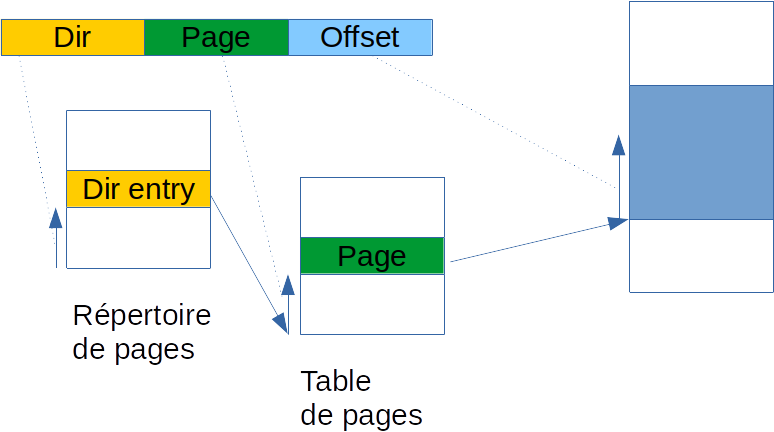
\includegraphics[width=0.8\textwidth]{adresse-lineaire}
$$
\caption{\label{Figure:addline}Structure d'une adresse linéaire.}
\end{figure} 
}
   Les bits de poids forts ({\tt Dir}) donnent la position dans le
répertoire de page de l'adresse d'une table de pages. Les bits
suivants ({\tt Page}) donnent la position dans dans cette table de
l'adresse d'une page en mémoire. Les derniers bits ({\tt Offset})
donnent alors la position recherchée dans cette page.

   Bien entendu, toutes les tables évoquées ici sont stoquées en
mémoire.


%-------------------------------------------------------------------------------
%      La mémoire virtuelle
%-------------------------------------------------------------------------------
\subsection{La mémoire virtuelle}

   Les processeurs Intel offrent depuis le 386 un mécanisme appelé
{\em pagination} permettant de définir un espace d'adressage {\em
virtuel} qui est réparti sur un espace d'adressage physique. Une
partie de cet espace physique peut être située ailleurs qu'en mémoire
centrale, ce qui permet de construire une mémoire virtuelle plus
grande que la mémoire réellement disponible.

   De plus, la gestion de la pagination peut être spécifique à chaque
tâche, ce qui permet de construire un système multitâche dans lequel
chaque tâche a une vision de l'espace mémoire qui lui est propre.

   Il y a donc deux problèmes à résoudre, que sont l'organisation de
la mémoire physique (et sa répartition entre les différentes tâches)
et l'organisation de la mémoire virtuelle vue par une tâche. Nous
allons voir comment ils sont résolus dans Manux, mais regardons
d'abord un peu comment la pagination est mise en \oe{}uvre.

%...............................................................................
%      Pagination
%...............................................................................
\subsubsection{Pagination}

   Le mécanisme de pagination des processeurs Intel permet, comme
l'illustre la figure \ref{Figure:Pagination}, de construire une
mémoire virtuelle, découpée en pages (de 4 Ko) à partir de pages
physiques situées ``n'importe où'' en mémoire physique (ou même sur un
autre support tel qu'un disque dur ou autre).

\note{
\begin{figure}[htbp]
$$
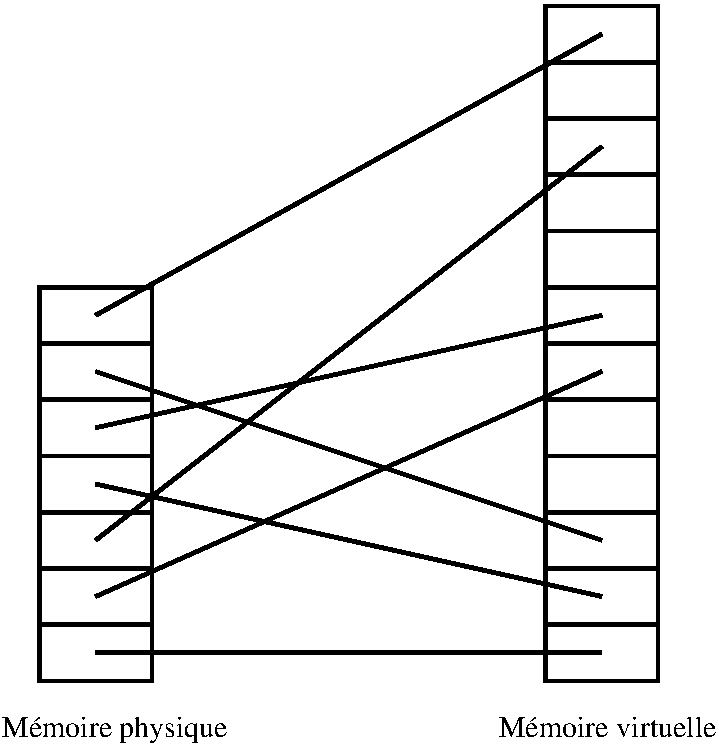
\includegraphics[width=0.5\textwidth]{Pagination}
$$
\caption{\label{Figure:Pagination}Principe de la pagination}
\end{figure} 
}
   Le processeur offre (via sa {\sc mmu}) des mécanismes évolués
permettant la mise en place de la pagination. La pagination est
activée en positionnant à un le bit 31 du registre {\sc cr0}.

   Lorsque la pagination est activée, le registre {\sc cr3} doit
contenir l'adresse (physique) d'une page mémoire contenant le {\em
répertoire de pagination} \index{Pagination!Répertoire de \ldots}.

%...............................................................................
%      Gestion de la mémoire physique
%...............................................................................
\subsubsection{Gestion de la mémoire physique dans ManuX}

   La mémoire physique est partagée entre une partie système et une
partie application. La première partie est dédiée à la gestion du
système et la seconde et utilisée pour satisfaire les besoins en
mémoire des différentes applications.

\note{
\begin{figure}[htbp]
$$
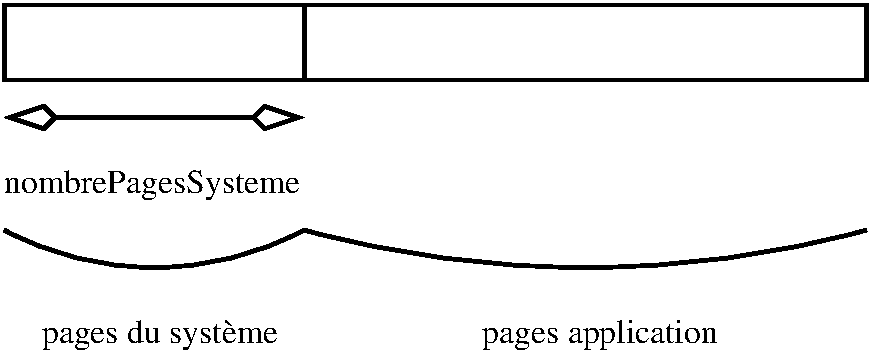
\includegraphics[width=0.5\textwidth]{MemoirePhysique}
$$
\caption{\label{Figure:MemoirePhysique}Structure de la mémoire physique}
\end{figure} 
}
   Au niveau système, la mémoire est gérée par page (une gestion plus
fine doit donc être implantée au niveau application, par le biais
des librairies).

%
%
%
\paragraph{Organisation de la mémoire physique}

   Traditionnellement, sur un PC, la mémoire physique est organisée
comme décrit par la figure \ref{etat-memoire-base}.

\note{
\begin{figure}[htbp]
$$
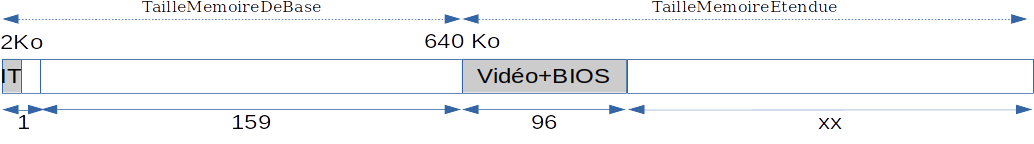
\includegraphics[width=\textwidth]{etat-memoire-base}
$$
\caption{\label{fig:etat-memoire-boot}État de la mémoire au démarage}
\end{figure} 
}
   Une partie est réservée pour le {\sc bios} et la vidéo, nous nous
garderons bien d'aller y lire ou écrire pour autre chose !
   
   L'état de cette mémoire à la fin du boot (décrit plus haut) est
donné  par la figure \ref{etat-memoire-boot-2} que nous redonnons ici.

\begin{figure}[htbp]
\includegraphics[width=\textwidth]{etat-memoire-boot}
\caption{\label{fig:etat-memoire-boot-2}État de la mémoire après le boot}
\end{figure} 

   Il est important de l'avoir en tête pour la suite afin de
déterminer quelles sont les zones que nous pouvos allouer et celles
qui ne doivent pas être utilisées.

%
%
%
\paragraph{Allocation de la mémoire}

   Chaque page mémoire peut être allouée à une tâche (ou au noyau) ou
libre (non allouée). C'est le tableau \lstinline!proprietairePage!
défini dans le fichier {\tt noyau/memoire.c} qui définit cela comme illustré par la figure
\ref{Figure:ProprietairePage}. Une page libre sera associée à un
propriétaire nul et une page allouée au système à la tâche 1.

\note{
\begin{figure}[htbp]
$$
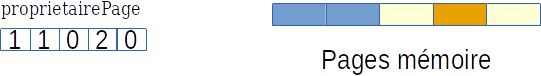
\includegraphics[width=0.5\textwidth]{proprietaire-page}
$$
\caption{\label{Figure:ProprietairePage}Définition de l'allocation des
  pages mémoire}
\end{figure} 
}
\subparagraph{Initialisation}



\subparagraph{Allocation}

   Deux fonctions permettent d'allouer une page mémoire, ce sont

\begin{lstlisting}{}
void * allouerPageSysteme();
void * allouerPage();
\end{lstlisting}

   qui permettent d'obtenir respectivement une page mémoire système et
une page mémoire application.

%...............................................................................
%
%...............................................................................
\subsection{Gestion fine de la mémoire dans le noyau}

   L'allocation de la mémoire physique page par page et importante,
mais il est également très utile de pouvoir allouer la mémoire avec
une granularité bien plus fine. Tous les sous-systèmes du noyau qui
ont besoin d'allocation dynamique manipulent des objets qui sont pour
la plupart bien plus petits qu'une page !

   On peut alors envisager deux grandes familles de techniques : un
allocateur ``généraliste''  (qui va fournir un service tel que le
malloc classique de la librairie C) ou un allocateur plus spécialisé
(qui permettra une gestion bien plus efficace d'un type d'objets
unique avec éventuellement un système d'initialisation, etc ...)

%...............................................................................
%  
%...............................................................................
\subsubsection{Un allocateur généraliste}

   Dans ManuX, un système d'allocation fine est implanté dans les
fichiers kmallc-zs.h et .c. Il utilise la technique des ``zones
siamoises'' ou buddy memory allocation system.

   Il fournit essentiellement les trois fonctions suivantes

void kmallocInitialisation();

void * kmalloc(size_t n);

void kfree(void * p);


%...............................................................................
%      Organisation de la mémoire virtuelle
%...............................................................................
\subsubsection{Organisation de la mémoire virtuelle}



%===============================================================================
%
%===============================================================================
\section{La librairie du noyau}

   Je vais décrire ici rapidement les outils fournis pour le noyau,
c'est-à-dire tout ce qui est codé dans le répertoire {\tt lib}.

%-------------------------------------------------------------------------------
%
%-------------------------------------------------------------------------------
\subsection{Le journal}

   Le journal permet d'archiver les messages émis par les différents
éléments du noyau grâce à la fonction \lstinline!printk()!
\index{printk()}.

   Le journal est défini dans le fichier {\tt include/journal.h} et implanté
dans le fichier {\tt lib/journal.c}.

%-------------------------------------------------------------------------------
%
%-------------------------------------------------------------------------------
\subsection{Le ramdisk}
 
   Le but du ramdisk est uniquement de nous permettre de valider
certains éléments du système, tels que le système de fichiers, sans
avoir besoin d'éléments complexes qui seront bien plus longs à mettre
en place et à tester, comme un pilote de disque dur ou de lecteur de
disquettes.

   Il permet de plus une certaine forme de communication avec le
système d'exploitation de développement puisqu'une image disque peut
être construite sur ce système avant d'être exploitée dans Manux-32.

%===============================================================================
%
%===============================================================================
\section{Les outils de synchronisation}

%-------------------------------------------------------------------------------
%
%-------------------------------------------------------------------------------
\subsection{Quel est le problème ?}

Registres, mémoire, ...

Monoprocesseur !

   Allez donc voir votre cours de systèmes d'exploitation !

   Imaginons un programme en cours d'exécution. Nous pouvons le voir
comme une séquence d'instructions en assembleur exécutées par le
processeur. Ce dernier utilise pour cela des variables qui sont dans
des registres et de la mémoire ; une telle exécution est appelée une
tâche, et nous appellerons celle-ci T1. 

   La figure suivante illustre cette exécution, représentée par la
flèche bleue.

premiere image

   Comme vous le savez, la tâche T1 peut être
interrompue, ce qui va conduire à l'exécution d'une autre séquence
d'instructions, typiquement le code la fonction de traitement (le {\em
  handler}) de l'interruption en question. À la fin de cette fonction
de traitement, l'exécution de la séquence initiale reprendra son
cours exactement là où il en était. Cela se fera probablement parce
que la dernière instruction de la fonction de traitement est
\lstinline!iret! ou un équivalent.

   La figure suivante illustre ce principe.

includegraphics(deuxieme image)

   Mais comment est-ce possible ? Pour exécuter correctement le
programme, le microprocesseur utilise des registres et de la mémoire,
nous l'avons dit, mais la fonction de traitement de l'interruption va
faire exactement la même chose ! Comment peut-on alors être sûr que le
retour au programme initial se fera vraiment dans les mêmes
conditions, y compris avec les valeurs inchangées dans les registres
et dans la mémoire ?

   Avant de discuter des éléments de réponse, nous allons élargir
davantage le problème.

   En effet, puisqu'il est possible d'interrompre la tâche T1
pendant quelques temps et d'y revenir ensuite, pourquoi ne
oas profiter de ce temps pour faire autre chose ? C'est exactement
cette idée qui va nous permettre de mettre en place du pseudo
parallélisme : plutôt que reprendre le cours de T1, nous pouvons
reprendre le cours d'une autre tâche, appelons la T2. Plus tard,
l'exécution de T2 sera probablement interrompue à son tour, et il sera
alors possible de reprendre le cours de T1 (ou d'une autre tâche T3
!). 

   La figure suivante illustre un tel mécanisme. Les raisons pour
lesquelles un tel fonctionnement peut êtr intéressant seront décrites
ailleurs. Les outils et techniques permettant de le réaliser sont
présentées dans le chapitre lié à l'ordonnancement.

ici troisieme image

   On comprend alors que la gestion de l'état des registres et de la
mémoire prend une autre dimension.
   
%-------------------------------------------------------------------------------
%
%-------------------------------------------------------------------------------
\subsection{Premières pistes : un peu de civisme}

   Une première réponse consiste à sauvegarder les registres dans la
pile (par des instructions \lstinline!push!) au début de la fonction
de traitement de l'interruption et à les restaurer à la fin de cette
fonction (grâce à des instructions \lstinline!pop!). Cela permet donc
de rêgler la question des registres sans altérer la pile qui est alors
elle aussi rendue dans le même état qu'avant l'interruption, \ldots

   Qu'en est-il des variables situées en mémoire ? La pile à une
gestion un peu spécifique, qui permet d'empiler des données durant le
traitement de l'interruption comme nous venons de l'évoquer. Les
données placées dans la pile peuve être manipulées sans conséquence
pour le programme qui a été interrompu, pour peu qu'elles soient
empilées puis dépilées par la fonction de traitement. La pile pourra
donc être utilisée pour stoquer des données temporaires durant le
traitement de l'interrruption.

   Cette première idée constitue une rêgle de ``bonne conduite'' que
l'on devra scrupuleusement respecter pour que le système puisse
fonctionner : les fonctions de traitement des interruptions devront
sauvegarder dans la pile les registres qu'elles sont susceptibles de
modifier (y compris les ``flags'' bien sûr) et les restaurer avant de
rendre la main.

%-------------------------------------------------------------------------------
%
%-------------------------------------------------------------------------------
\subsection{Gestion du multi tâches : un peu d'organisation}

   La bonne conduite des fonctions de traitement des interruptions est
donc une nécessité pour un bon fonctionnement d'un système monotâche,
mais elle ne saurait suffir sur un système multitâche. Il faut en
effet maintenant être capable, avant de reprendre l'exécution de la
tâche T2, par exemple, de restaurer l'état des registres tel qu'ils
étaient lorsque cette tâche avait été interrompue, et non tels qu'ils
étaient lorsque la dernière tâche en cours (la tâche T1 par exemple a
été interrompue).

   Le noyau va donc devoir mettre en place des techniques
(potentiellement avec l'aide su matériel) lui permettant de restaurer
les registres dans l'état convenable avant de reprendre l'exécution
d'une tâche. Dans la figure précédente, c'est donc avant l'étape 5 que
le système doit d'assurer que les registres sont bien dans l'état dans
lequel les avait laissés la tâche T2, et non la tâche T1.

%-------------------------------------------------------------------------------
%
%-------------------------------------------------------------------------------
\subsection{Et la mémoire dans tout ça ?}

   Nous ne nous sommes intéressés jusque là qu'aux variables qui
étaient contenues dans des registres, mais nos programmes utilisent
aussi la mémoire pour stocker les variables. Comment la cohérence
est-elle assurée pour elle ?

%...............................................................................
%
%...............................................................................
\subsubsection{Une première solution : chacun chez soi !}

   La première idée, bien sûr, est de s'assurer que chaque tâche ait
accès à une zone mémoire qui lui soit réservée. Si elle et elle seule
peut y accéder, aucun risque d'incohérence, et tout va bien, ...

   Comment assurer qu'un tel principe fonctionne correctement ? Il y a
évidemment deux possibilités : on fait confiance aux tâches (à leurs
auteurs et leurs utilisateurs), ou on met en place des mécanismes de
protection.

   La première solution peut être acceptable dans des environnements
maîtrisés : si vous êtes l'auteur de l'intégralité du système, vous
savez que vous avez programmé vos applications en respectant les
rêgles. 

   Dans un cadre plus général, il faudra passer par la seconde
solution. C'est alors le noyau qui va devoir attribuer la mémoire aux
différentes tâches et les empêcher, avec l'aide du matériel, d'aller
lire ou écrire ailleurs. Je vous parle de cela dans le chapitre dédié
à la gestion de la mémoire, ...

%...............................................................................
%
%...............................................................................
\subsubsection{Le retour du civisme}

   L'autre solution permettant d'assurer la cohérence du contenu de la
mémoire est à nouveau, comme pour les registres, de définir ``quelques
rêgles simples'' et de s'y tenir. L'nesemble des outils de
synchronisation dont vous avez entendu parlé dans vos cours, et
notemment ceux dont je vais parler ici, permettent de mettre en place
ces rêgles simples.

   Il est en revanche cette fois ci plus délicat pour le système de
mettre en place des outils cohercitifs obligeant les tâches à
respecter ces rêgles. Cependant, comme nous allons le voir, ce n'est
généralement pas nécessaire, car on va se placer dans des situations
dans les lesquelles on sait pouvoir faire confiance aux différentes
tâches.

%...............................................................................
%
%...............................................................................
\subsubsection{Quel modèle choisir ?}

   Vous l'avez compris, malin que vous êtes, les deux techniques que
je viens d'évoquer correspondent à deux modèles de gestion de la
mémoire

begin itemize
   item la mémoire peut être partagée entre les différentes tâches
   qui s'exécutent sur le système ;
   item la mémoire peut être réservée à chaque tâche.
end itemize

   La mémoire réservée est une façon un peu extrème de répondre aux
problèmes de cohérence puisqu'ils disparaissent complètement, mais
elle ne permet pas aux différentes tâches de communiquer (il faudra
donc trouver d'autres solutions pour cela).
   C'est une technique assez largement utilisée dans les systèmes
   généraux multitâches. Elle est illustrée par la figure suivante.

   ici figure

   La technique de la mémoire partagée est plus simple à mettre en
oeuvre, et permet aux tâches de communiquer entre elles, mais elle va
nécessiter la mise en place d'outils de synchronisation pour assurer
la cohérence, et elle ne permet pas de protéger une tâches contre les
actions malveillantes ou accidentelles des autres tâches. Elle est
illustrée par la figure suivante.

   Ici figure

   Pour marier les avantages des deux techniques, un système de type
Unix les implante toutes les deux comme illustré par la figure
suivante.

ici figure

   L'idée est qu'une tâche (oui, je sais, le terme utilisé ici est
processus) va disposer d'une partie de la mémoire pour faire ce
qu'elle veut, et que lorsqu'elle va avoir besoin des services du
noyau, elle s'exécuter en mode protégé et pouvoir accéder ainsi, via
le code du noyau, à une zone mémoire commune. C'est donc dans le code
du noyau que seront utilisés les outils de synchronisation assurant la
cohérence.

   Pour résumer, sur un système classique de type Unix utilisant des
``processus lourds'', seul le code du noyau doit s'inquiéter des
problèmes de synchronisation. Sur un système sans outils matériel de
protection de la mémoire, c'est plus compliqué, ...

   Notons tout de même qu'un système de type Unix peut également
implanter des ``processus légers'' ou threads (par exemple
conformément à la norme POSIX dont j'ai oublié le numéro). On se
retrouve alors avec une situation comme celle de la figure suivante.

ici fugure

   Dans ce cas, le code d'une application qui utilise cette
fonctionnalité doit lui aussi être instrumenté par des outils de
synchronisation de sorte à assurer la cohérence des données.

Résumé des situation problématiques sur un système monoprocesseur

   Si nous envisageons un système de type Unix sur une machine
monoprocesseur, qui implante des processus lourds avec une isolation
de la mémoire assurée par une MMU, quelles sont finalement les
situations à prendre en compte ? Il y en a essentiellement deux :

   Un traitement en court peut être préempté par une
   interruption. Cette situation peut être exceptionnellement évitée
   au besoin (en interdisant brièvement certaines interruptions). Ses
   conséquences peuvent également être maîtrisées par le fait que le
   traitement d'une interruption sera aussi limité que possible. Des
   outils de sycnhronisation restent cependant nécessaires, avec une
   contrainte spécifique : il est inenvisageable de mettre en attente
   le code de traitement d'une interruptions !

   Une tâche en train d'effectuer une action dans le noyau (en
   particulier par le biais d'un appel système) peut être interrompue
   pour passer la main à une autre tâche qui va à son tour effectuer
   un traitement dans le noyau. Une première approche, relativement
   simple, consiste à interdire la présence de plus d'une tâche dans
   le noyau à tout instant (on parle de verouillage globale du noyau,
   ou ``big kernel lock''). Une solution plus subtile (et bien plus
   efficace sur un système multiprocesseur) sera de protéger chaque
   variable (ou sous-système) sensible du noyau par des outils de
   synchroniation. 

%===============================================================================
%      les outils de synchronisation
%===============================================================================
\section{L'implantation dans ManuX}

   ManuX implante utilise un modèle de mémoire allouée en mode
utlisateur et partagée dans le noyau. En l'absence de gestion de la
mémoire fondée sue la MMU, l'usage exclusif de la mémoire allouée en
mode utilisateur est fondé sur le civisme du code applicatif.

   Dans le noyau, c'est une autre histoire ; les données peuvent être
manipulées par plusieurs tâches, et des outils de synchronisation
doivent donc être mis en place.


   
   Les moyens de synchronisation entre tâches actuellement disponibles
sont 

\begin{itemize}
   \item les opérations atomiques ;
   \item les exclusions mutuelles.
\end{itemize}

%-------------------------------------------------------------------------------
%      Opérations atomiques
%-------------------------------------------------------------------------------
\subsection{Opérations atomiques}

   Les opérations élémentaires de synchronisation sont définies dans
le fichier {\tt atomique.h}. Elles se basent sur le type
\lstinline!Atomique! et les opérations qui lui sont associées. A part
l'initialisation et la consultation, l'opération importante est la
suivante

\begin{lstlisting}{}
booleen atomiqueTestInit(volatile Atomique * atom, uint32 val, uint32 cond);
\end{lstlisting}

   Elle compare la valeur de l'\lstinline!Atomique! avec
\lstinline!cond! et, en cas d'égalité, affecte l'\lstinline!Atomique!
avec la valeur \lstinline!val! et renvoie \lstinline!TRUE!, sinon elle 
ne fait rien et renvoie \lstinline!FALSE!. Ce qui est important, bien
sur, c'est que la comparaison et l'éventuelle affectation soient
réalisées de façon {\em atomique}.

%-------------------------------------------------------------------------------
%      Exclusions mutuelles
%-------------------------------------------------------------------------------
\subsection{Exclusions mutuelles}

   Les variables d'exclusion mutuelle permettent d'assurer que l'accés
à une ressource (typiquement une section de code critique) se fait de
façon exclusive entre les tâches.

   Le fichier {\tt atomique.h} définit le type et les fonctions
suivants 

\begin{lstlisting}{}
typedef struct _ExclusionMutuelle {
   Atomique   verrou;
   ListeTache tachesEnAttente;
} ExclusionMutuelle;

void initialiserExclusionMutuelle(ExclusionMutuelle * em);
void entrerExclusionMutuelle(ExclusionMutuelle * em);
void sortirExclusionMutuelle(ExclusionMutuelle * em);
\end{lstlisting}

   Naturellement, comme leurs noms l'indiquent, les trois
sous-programmes permettent respectivement d'initialiser une variable
d'exclusion mutuelle, de prendre une exclusion mutuelle et de libérer
une exclusion mutuelle.



%===============================================================================
%      Interface système
%===============================================================================
%\section{Interface système}

%   L'interface entre le système et les applications est réalisée par
%le biais des appels système.

%===============================================================================
%      L'ordonnancement des tâches
%===============================================================================
\section{L'ordonnancement des tâches}

   Le scheduler est l'entité chargée de la mise en \oe{}uvre de
l'ordonnancement. Aussi étrange que cela puisse paraitre, il est
implanté sous la forme d'un processus. En fait, chaque fois qu'il est
nécessaire de changer de tâche active (lorsque le quantum de temps
alloué à celle en cours est révolu, ou qu'elle se bloque sur une
entrée/sortie), le système bascule vers la tâche scheduler, qui se
charge alors d'élire la prochaine tâche et de l'activer.

   Le corps du scheduler se résume alors à une boucle folle qui ne
fait qu'appeler le sous-programme {\tt basculerTache()} chargé de
l'élection de la prochaine tâche.

   Naturellement, la tâche de l'ordonnanceur n'est pas stockée dans la
liste des tâches actives du système.

%===============================================================================
%      Le système de fichiers
%===============================================================================
\section{Le système de fichiers}
%===============================================================================
%
%===============================================================================
\section{Introduction}

   Nous allons décrire ici les outils permettant de définir et
manipuler les fichiers ainsi que les interfaces permettant d'accéder à
des fichiers.

   Nous verrons également que ces interfaces permettent l'accès à d'autres outils
d'échange d'information. C'est en effet une pratique classique que de
proposer une interface la plus simple et la plus homogène possible à
tous les outils de stockage et d'échange de données.

   Nous allons commencer par essayer de définir clairement les deux
principales structures de données classiquement utilisées : le {\em
  noeud d'index} et le {\em fichier ouvert}.

   La première de ces structures donne des informations sur la
structure et les propriétés du fichier ; c'est au travers d'elle que
nous pourrons savoir où se trouve physiquement le fichier, à qui il
appartient, qu'est-ce qu'un utilisateur a le droit d'en faire, etc
\ldots

   La seconde contient des informations plus dynamiques sur un fichier
qui est manipulé par une tâche. On y trouvera donc par exemple la
position actuelle dans le fichier.

   Une analogie simple nous permet de dire que le n\oe{}ud d'index
nous permet de savoir qu'un livre est situé dans la troisième rangée
de la deuxième étagère (et qu'il est interdit d'écrire sur le livre
!), la où le fichier ouvert contient par exemple un marque page
positionné à la prochaine page qu'un utilisateur s'apprète à lire.

%===============================================================================
%
%===============================================================================
\section{Notion de noeud d'index}

   La structure permettant de décrire les propriétés d'un fichier est
classiquement appelée {\em n\oe{}ud d'index}, ou plus souvent {\em
  inode} (pour {\em index node}).

%-------------------------------------------------------------------------------
%
%-------------------------------------------------------------------------------
\subsection{Dans ManuX}

   ManuX définit la structure \lstinline!NoeudI! et les fonctions
associées  dans le fichier \fichier{include/manux}{noeudi}{h}. Les
fonctions sont implantées dans le fichier \fichier{sf}{noeudi}{c}.

   Une chose importante à avoir en tête est le fait qu'un fichier
décrit par un NoeudI peut être de diverses natures et qu'il est donc
important de garder trace d'informations permettant de savoir comment
le manipuler.

   La structure \lstinline!NoeudI! intègre en particulier les champs
suivants~:

\begin{itemize}
   \item \lstinline!methodesFichier! fourni les fonctions de
     manipulation d'un fichier du type concerné.
   \item \lstinline!prive! est un pointeur vers des données
     spécifiques au type du fichier et permettant de définir des
     propriétés spécifiques du fichier.
\end{itemize}
    
\subsubsection{Les méthodes de manipulation des fichiers}

%===============================================================================
%
%===============================================================================
\section{Description d'un fichier ouvert}

%-------------------------------------------------------------------------------
%
%-------------------------------------------------------------------------------
\subsection{Dans ManuX}

   Dans ManuX, un fichier ouvert est décrit dans la structure
\lstinline!fichier! qui contient en particulier les données suivantes
   
\begin{itemize}
   \item \lstinline!noeudI! 
   \item \lstinline!prive! est un pointeur vers des données
     spécifiques au type du fichier et permettant de conserver trace
     de l'état du fichier.
\end{itemize}
   

%===============================================================================
%
%===============================================================================
\section{Outils de base de manipulation des fichiers}

%-------------------------------------------------------------------------------
%
%-------------------------------------------------------------------------------
\subsection{Interface utilisateur}

   L'interface fournie à l'espace utilisateur est généralement simple
et la plus abstraite possible. Elle passe par un certain nombre
d'appels système permettant en particulier d'ouvrir, de lire, d'écrire
et de fermer un fichier.

%-------------------------------------------------------------------------------
%
%-------------------------------------------------------------------------------
\subsection{Dans le noyau}

%-------------------------------------------------------------------------------
%
%-------------------------------------------------------------------------------
\subsection{Dans ManuX}

   ManuX définit une interface utilisateur classique fondée sur
quelques appels systèmes inspirés de ce que l'on trouve dans un
système Unix.

%...............................................................................
%
%...............................................................................
\subsubsection{L'interface}

%
%
%
\paragraph{Ouverture d'un fichier}

L'ouverture d'un fichier se fait à l'aide de l'appel système
\lstinline!UNDEFINED!.

%
%
%
\paragraph{Lecture dans un fichier}

L'appel système \lstinline!lire! est défini dans le fichier
\fichier{usr/include}{stdio}{h} de la façon suivante~:

\begin{lstlistings}
int lire(int fd, void * buffer, int nb);
\end{lstlistings}

%
%
%
\paragraph{Écriture dans un fichier}

%...............................................................................
%
%...............................................................................
\subsubsection{Dans le noyau}

%
%
%
\paragraph{Lecture dans un fichier}

   L'implantation de l'appel système de lecture est réalisée dans la
fonction \lstinline!sys_lire()! implantée dans le fichier
\fichier{sf/fichier}{c}. L'appel système est défini dans la fonction
\lstinline!sfInitialiser() du même fichier.

   Cette fonction peut servir en particulier à mettre en place des
contrôles de sécurité. Elle se contente pour le moment de faire appel
à la fonction \lstinline!fichierLire()! qui est en charge d'aiguiller
vers la fcontion de lecture spécifique au type du fichier ciblé.

%===============================================================================
%
%===============================================================================
\section{Un exemple : les consoles}

   Je ne vais pas revenir ici sur l'implantation des consoles, déjà
décrite avec brio dans le chapitre qui leur est dédié. Regardons
simplement comment elles se retrouvent affublées d'une interface de
type fichier.

   Dans le fichier \fichier{lib}{console}{c}, les fonctions de
manipulation d'une console sont définies de la façon suivante

\begin{lstinline}
/**
 * @brief Déclaration des méthodes permettant de traiter une console
 * comme un fichier
 */
MethodesFichier consoleMethodesFichier = {
   .ouvrir = consoleOuvrir,
   .ecrire = consoleEcrire,
   .lire = consoleFichierLire
};
\end{lstinline}

%-------------------------------------------------------------------------------
%
%-------------------------------------------------------------------------------
\subsection{La fonction d'écriture}

   La fonction \lstinline!consoleEcrire()! est alors simplement
constituée d'un appel à la fonction d'affichage dans la console visée,
dont un pointeur est obtenu via le champ privé.

   ATTENTION ! il faut aller le chercher via le noeudI, ce qui n'est
   pas le cas pour le moment !!!
   
%===============================================================================
%
%===============================================================================
\section{Les tubes de communication}

Les méthodes de manipulation


%===============================================================================
%
%===============================================================================
\appendix

%-------------------------------------------------------------------------------

\printindex
\end{document}

